\renewcommand{\theequation}{\theenumi}
\renewcommand{\thefigure}{\theenumi}
\begin{enumerate}[label=\thesubsection.\arabic*.,ref=\thesubsection.\theenumi]
\numberwithin{equation}{enumi}
\numberwithin{figure}{enumi}
%
\item Trace the parabola:
\begin{align}
	(x-4y)^2=51y
\end{align}
%
\solution
Expanding the given equation, we have,
\begin{align}
    x^2 -8xy +16y^2 -51y =0 \label{eq:solutions/41/1/eq:1}
\end{align}
The general equation of second degree is given by
\begin{align}
	ax^2+2bxy+cy^2+2dx+2ey+f=0 \label{eq:solutions/41/1/gen_eq}
\end{align}
and can be expressed as
\begin{align}
	\vec{x}^T\vec{V}\vec{x}+2\vec{u}^T\vec{x}+f=0 \label{eq:solutions/41/1/conic_eq}
\end{align}
where
\begin{align}
	\vec{V} &= \vec{V}^T = \myvec{a & b \\ b & c}
	\\
	\vec{u}^T &= \myvec{d & e}
\end{align}
From equation \eqref{eq:solutions/41/1/eq:1} , we get
\begin{align}
	\vec{V} &= \myvec{1 & -4\\-4 & 16}\label{eq:solutions/41/1/eq:2}\\
	\vec{u} &= \myvec{0\\-\frac{51}{2}}\label{eq:solutions/41/1/eq:3}\\ 
	f &= 0 \label{eq:solutions/41/1/eq:4}
\end{align}
Expanding the determinant of $\vec{V}$ we observe, 
\begin{align}
	\mydet{1 & -4\\-4 & 16} = 0
\end{align}
Therefore, \eqref{eq:solutions/41/1/eq:1} is a parabola.

The characteristic equation of $\vec{V}$ is given as follows,
\begin{align}
		\mydet{\lambda\vec{I}-\vec{V}} = \mydet{\lambda-1&4\\ 4&\lambda-16} &= 0\\
		\implies \lambda^2-17\lambda &= 0\label{eq:solutions/41/1/eq:5}
\end{align}
The eigenvalues are given by
\begin{align}
		\lambda_1=0, \lambda_2=17\label{eq:solutions/41/1/eq:6}    
\end{align}
For $\lambda_1 = 0$, the eigen vector $\vec{p}$ is given by 
\begin{align}
		\vec{V}\vec{p} = 0
\end{align}

Row reducing $\vec{V}$ 
\begin{align}
		\myvec{1&-4\\-4&16}\xleftrightarrow[R_2=R_2+R_1]{R_2=R_2/4}\myvec{1&-4\\0&0}\\
		\implies\vec{p}_1=\frac{1}{\sqrt{17}}\myvec{-4\\-1} \label{eq:solutions/41/1/eq:7}
\end{align}
Similarly, 
\begin{align}
		\vec{p}_2=\frac{1}{\sqrt{17}}\myvec{-1\\4} \label{eq:solutions/41/1/eq:8}
\end{align}

Thus,
\begin{align}
		\vec{P}&=\myvec{\vec{p_1}&\vec{p_2}}=\frac{1}{\sqrt{17}} \myvec{-4 & -1\\ -1 & 4} 
\end{align}
The equation of the parabola is:
\begin{align}
		\vec{y^T}\vec{D}\vec{y}&=-2\eta\myvec{1&0}\vec{y}
\end{align}
where
\begin{align}
		\eta=\vec{u}^T\vec{p_1}=\frac{51}{2\sqrt{17}}
\end{align}
and focal length of the parabola is given by 
\begin{align}
	\frac{\abs{2\vec{u}^T\vec{p_1}}}{\lambda_2}	= \frac{3}{\sqrt{17}}
\end{align}

Now,
\begin{align}
		\myvec{\vec{u^T}+\eta\vec{p_1^T} \\ \vec{V}}\vec{c}=
		\myvec{-f \\ \eta\vec{p_1}-\vec{u}} \label{eq:solutions/41/1/eq:9}
\end{align}
using equations \eqref{eq:solutions/41/1/eq:2}, \eqref{eq:solutions/41/1/eq:3} and \eqref{eq:solutions/41/1/eq:9}
\begin{align}
	\myvec{-6& -27 \\ 1 & -4 \\  -4 & 16 }\vec{c}=\myvec{0 \\ -6\\ 24} 
\end{align}

Forming the augmented matrix and row reducing it:
\begin{align}
		\myvec{-6 & -27 & 0\\1 & -4 & -6 \\-4 & 16 & 24}\\
		\xleftrightarrow[]{R_3\leftarrow R_3+ 4R_2} 
		\myvec{-6 & -27 & 0\\1 & -4 & -6 \\0 & 0 &0 }\\
		\xleftrightarrow[]{R_1\leftarrow R_1/(-6)} 
		\myvec{1 & 9/2 & 0\\1 & -4 & -6\\0 & 0 &0 }\\
		\xleftrightarrow[]{R_2\leftarrow R_2-R_1} 
		\myvec{1 & 9/2 & 0\\0 & -17/2 & -6 \\0 & 0 &0 }\\
		\xleftrightarrow[]{R_2\leftarrow (-\frac{2}{17})R_2}
		\myvec{1 & 9/2 & 0\\0 & 1 & 12/17\\0 & 0 &0}\\ 
		\xleftrightarrow[]{R_1\leftarrow R_1 -(\frac{9}{2})R_2}
		\myvec{1 & 0 & -54/17\\0 & 1 & 12/17 \\0 & 0 &0}
\end{align}

Thus the vertex is:
\begin{align}
	&\vec{c}= \myvec{-\frac{54}{17}\\ \frac{12}{17}} \\
	&\approx \myvec{-3.18\\ 0.71}
\end{align}

\begin{figure}[!htbp]
	\centering
	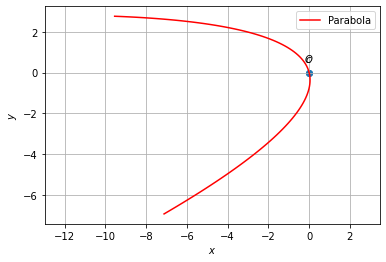
\includegraphics[width =\columnwidth]{solutions/41/1/parabola plot.png}
	\caption{Parabola }
	\label{eq:solutions/41/1/fig:1}
\end{figure}	



%
\item 	Trace the curve 
	\begin{align}
	\left(x-y\right)^2 = x+y+1
	\label{eq:solutions/41/2/eq0}
	\end{align}
%
\solution
	
	We have given equation as :
	\begin{align}
\left(x-y\right)^2 = x+y+1
\end{align}	
\begin{align}
\implies x^2  -2xy + y^2 -x - y -1 = 0
\label{eq:solutions/41/2/eq1}
\end{align}
The general equation of second degree is given by
\begin{align}
ax^2+2bxy+cy^2+2dx+2ey+f=0 \label{eq:solutions/41/2/eq2}
\end{align}
and can be expressed as
\begin{align}
\vec{x}^T\vec{V}\vec{x}+2\vec{u}^T\vec{x}+f=0 \label{eq:solutions/41/2/eq3}
\end{align}
where
\begin{align}
\vec{V} &= \vec{V}^T = \myvec{a & b \\ b & c}
\\
\vec{u}^T &= \myvec{d & e}
\end{align}

Comparing \eqref{eq:solutions/41/2/eq1} with \eqref{eq:solutions/41/2/eq2}, we get

\begin{align}
\vec{V} &= \vec{V}^T = \myvec{ 1 &  -1 \\ -1 & 1 }
\\
\vec{u}^T &= \myvec{-\frac{1}{2} & - \frac{1}{2}}
\\
f &= -1
\end{align}


Expanding the determinant of V we observe,
\begin{align}
\abs{\vec{V}} = \mydet{1 & -1 \\ -1 & 1} = 0 \label{eq:solutions/41/2/eq10}
\end{align}
Also
\begin{align}
\mydet{\vec{V} & \vec{u} \\ \vec{u}^T & f} = 
\mydet{
1 & -1 & -\frac{1}{2} \\ 
-1 & 1 & -\frac{1}{2} \\ 	
-\frac{1}{2} & -\frac{1}{2} & -1}
\neq 0
\label{eq:solutions/41/2/eq11}
\end{align}

Hence from \eqref{eq:solutions/41/2/eq10} and \eqref{eq:solutions/41/2/eq11} we conclude
that given equation is an parabola.The characteristic equation of $\vec{V}$ is given as
follows,


\begin{align}
\mydet{\lambda \vec{I}-\vec{V}} = \mydet{\lambda -1 & -1 \\ -1 & \lambda - 1} &= 0
\\
\implies \left(\lambda - 1 \right)^2 -1 &= 0
\label{eq:solutions/41/2/eq12}
\end{align}
The eigenvalues are the roots of \eqref{eq:solutions/41/2/eq12} given by
\begin{align}
\lambda_1 = 0, \lambda_2 = 2
\label{eq:solutions/41/2/eq13}
\end{align}
The eigenvector $\vec{p}$ is defined as:
\begin{align}
\vec{V} \vec{p}&= \lambda \vec{p}
\\
\implies \brak{\lambda\vec{I}-\vec{V}}\vec{p} &=0
\end{align}
where $\lambda$ is the eigenvalue.  For $\lambda_1$ = 0,
\begin{align}
\vec{V} \vec{p}&=0
\end{align}
Row reducing $\vec{V}$ yields,
\begin{align}
 \myvec{ 1 & -1 \\ -1 & 1} 
\xleftrightarrow{R_2\leftarrow R_2+R_1} 
\myvec{
	1 &  -1 \\ 0 & 0 
} 
\label{eq:solutions/41/2/eq18}
\end{align}

  Similarly, the eigenvector corresponding to $\lambda_2$ can be obtained as
  
  \begin{align}
  \brak{\lambda_2\vec{I}-\vec{V}}
  = \myvec{ 1 & 1 \\ 1 & 1} 
  \xleftrightarrow{R_2\leftarrow R_2 - R_1}
  \myvec{
  	1 & 1   \\ 0 & 0 
  }
  \label{eq:solutions/41/2/eq19}
  \end{align}
  
  
  

It is easy to verify that 
\begin{align}
\vec{V} &= \vec{P}\vec{D}\vec{P}^{-1}=\vec{P}\vec{D}\vec{P}^T \quad \because \vec{P}^{-1} = \vec{P}^{T} \label{eq:solutions/41/2/eq:solutions/41/ex1/ellipse_spectrum_eq}
\\
\text{or, } \vec{D} &= \vec{P}^T\vec{V}\vec{P}
\end{align}


From equation \eqref{eq:solutions/41/2/eq18} and \eqref{eq:solutions/41/2/eq19}, we have
\begin{align}
\vec{p_1} =  \frac{1}{\sqrt{2}} \myvec{1 \\ 1} 
\text{and},  \vec{p_2} =  \frac{1}{\sqrt{2}} \myvec{1 \\ -1} 
\end{align}
Thus, the eigenvector rotation matrix and the
eigenvalue matrix are 
\begin{align}
\vec{P} &= \frac{1}{\sqrt{2}} \myvec{ \vec{p_1} & \vec{p_2}} = \frac{1}{\sqrt{2}} \myvec{ 1 & 1 \\ 1 & -1} \\
 \vec{D} &= \myvec{0 & 0 \\ 0 & 2} 
\end{align}

\begin{figure}[htb!]	
	\centering	
	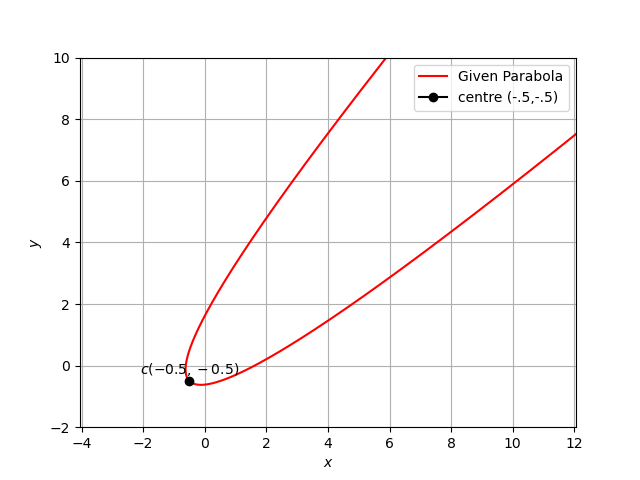
\includegraphics[width=\columnwidth]{./solutions/41/2/parabola.png}	
	\caption{Parabola with the center c}
	\label{eq:solutions/41/2/fig1}	
\end{figure}

The focal length of the parabola is
given by
\begin{align}
\frac{\mydet{2{\vec{u}}^T\vec{p_1}}}{\lambda_2 } = \frac{\sqrt{2}}{2} = \sqrt{2}
\end{align}
and its equation is
\begin{align}
\vec{y}^T\vec{D}\vec{y} = -2 \eta\myvec{1 & 0 }\vec{y}
\end{align}
where,
\begin{align}
\eta = \vec{u}^T\vec{p_1} = - \frac{1}{\sqrt{2}}
\end{align}

\begin{align}
\myvec{\vec{u}^T + \eta\vec{p_1}^T \\ \vec{V}}\vec{c} = \myvec{-f \\ \eta\vec{p_1} - \vec{u}} 
\end{align}
\begin{align}
\implies \myvec{ -1 & -1   \\ 1 & -1 \\ -1 & 1 }\vec{c} = \myvec{1 \\ 0 \\ 0}
\end{align}
Forming the augmented matrix and row reducing
it:


%\begin{align}
%\myvec{-1  &  -1 &  1 \\   1 & -1 &  1 \\  -1 & 1 & 0}  \label{eq:solutions/41/2/2.30}
%\end{align}

\begin{align}
\myvec{-1  &  -1 &  1 \\   1 & -1 &  1 \\  -1 & 1 & 0}  \label{eq:solutions/41/2/2.30}
\xleftrightarrow[]{R_2 \leftarrow R_2+R_1  }
%
\myvec{
-1 & -1 & 1 \\ 0 & -2 & 1 \\ -1 & 1 & 0  
} 
\xleftrightarrow[R_1 \leftarrow -1R_1] {R_3 \leftarrow  R_3 - R_1}  \nonumber  \\
%
\myvec{
1 & 1 & -1 \\ 0 & -2 & 1 \\ 0 & 2 & -1 
}
\xleftrightarrow[]{R_3 \leftarrow R_3 +R_2 } 
%	
\myvec{
1 & 1 & -1 \\ 0 & -2 & 1 \\ 0 & 0 & 0 
} \nonumber   \\
\xleftrightarrow[R_1 \leftarrow R_1 -R_2]{R_1 \leftarrow \frac{R_1}{-2}} 
\myvec{
1 & 0 & -\frac{1}{2} \\ 0 & 1 & - \frac{1}{2} \\ 0 & 0 & 0
}
\end{align}
So,
\begin{align}
\vec{c} = \myvec{ -\frac{1}{2} \\ -\frac{1}{2}  } \label{eq:solutions/41/2/2.31}
\end{align}







%
\item Trace the parabola
\begin{align}
    (4x+3y+15)^2=5(3x-4y)
\end{align}
%
\solution
%
The given equation can be rewritten as
\begin{align}\label{eq:solutions/41/4/eq:quadraticparabola}
    16x^2+24xy+9y^2+105x+110y+225 = 0
\end{align}
Comparing this to the standard equation,
%\vec{x}^T\vec{V}\vec{x}+2\vec{u}^T\vec{x}+f = 0
\begin{align}
    \vec{V} = \vec{V}^T = \myvec{16 & 12\\12 & 9}, \quad \vec{u} = \myvec{\frac{105}{2} \\ 55}, \quad f = 225 \label{eq:solutions/41/4/eq:Vufvals}
\end{align}
The characteristic equation of $\vec{V}$ is given as
\begin{align}
    \mydet{\lambda\vec{I}-\vec{V}} = 0\\
    \implies \mydet{\lambda-16 & -12 \\ -12 & \lambda-9} = 0\\
    \implies \lambda^2 -25\lambda = 0 \label{eq:solutions/41/4/eq:lambdaeq}
\end{align}
The eigenvalues are the roots of the equation \eqref{eq:solutions/41/4/eq:lambdaeq}, which are as follows :
\begin{align}
    \lambda_1 = 0, \quad \lambda_2 = 25 \label{eq:solutions/41/4/eq:eigenval}
\end{align}
The eigen vector $\vec{p}$ is defined as, 
\begin{align}
    \vec{V}\vec{p} &= \lambda\vec{p}\\
    \implies(\lambda\vec{I}-\vec{V})\vec{p}&=0
\end{align}
For $\lambda_1=0$
\begin{align}
    (\lambda_1\vec{I}-\vec{V}) = \myvec{-16 & -12\\-12 & -9}\xleftrightarrow[R_2\leftarrow R_2-3R_1]{R_1\leftarrow \frac{1}{4}R_1}\myvec{-4 & -3\\0 & 0}
\end{align}
\begin{align}
    \implies\vec{p_1}&=\frac{1}{5}\myvec{-3\\4}\label{eq:solutions/41/4/eq:p1val}
\end{align}
For $\lambda_2=25$
\begin{align}
    (\lambda_2\vec{I}-\vec{V}) = \myvec{9 & -12\\-12 & 16}\xleftrightarrow[R_2\leftarrow R_2+4R_1]{R_1\leftarrow \frac{1}{3}R_1}\myvec{3 & -4\\0 & 0}
\end{align}
\begin{align}
    \implies\vec{p_2}=\frac{1}{5}\myvec{4\\3}\label{eq:solutions/41/4/eq:p2val}
\end{align}
So, using Eigenvalue decomposition, $\vec{P}^T\vec{V}\vec{P}=\vec{D}$, where
\begin{align}
    \vec{P} = \frac{1}{5}\myvec{-3 & 4\\4 & 3}\\
    \vec{D} = \myvec{\lambda_1 & 0\\0 & \lambda_2} = \myvec{0 & 0\\ 0 & 25}
\end{align}
Then, for the parabola
\begin{align}
    \text{focal length} = \abs{\frac{2\eta}{\lambda_2}} \label{eq:solutions/41/4/eq:focallen}\\
    \eta = \vec{p}_1^T\vec{u} = \frac{25}{2}\label{eq:solutions/41/4/eq:etaval}\\
    \intertext{Substituting values from \eqref{eq:solutions/41/4/eq:etaval} and \eqref{eq:solutions/41/4/eq:eigenval} in \eqref{eq:solutions/41/4/eq:focallen}, we get}
    \text{focal length} = 1
\end{align}
The standard equation of the parabola is given by
\begin{align}
    \vec{y}^T\vec{D}\vec{y} = -2\eta\myvec{1 & 0}\vec{y}
\end{align}
And the vertex $\vec{c}$ is given by
\begin{align}
    \myvec{\vec{u}^T + \eta\vec{p}_1^T \\ \vec{V}}\vec{c} = \myvec{-f \\ \eta\vec{p}_1 - \vec{u}} \label{eq:solutions/41/4/eq:c}
\end{align}
Substituting values from \eqref{eq:solutions/41/4/eq:Vufvals},\eqref{eq:solutions/41/4/eq:etaval},\eqref{eq:solutions/41/4/eq:p1val} in \eqref{eq:solutions/41/4/eq:c},
\begin{align}
    \myvec{45 & 65\\16 & 12\\12 & 9}\vec{c} = \myvec{-225\\-60\\-45}
\end{align}
To find $\vec{c}$, performing row reduction on the augmented matrix as follows:
\begin{align}
    \myvec{45 & 65 & -225\\16 & 12 & -60\\12 & 9 & -45}\xleftrightarrow[R_1\leftarrow \frac{1}{45}R_1]{R_3\leftarrow R_3-\frac{3}{4}R_2}\myvec{1 & \frac{13}{9} & -5\\16 & 12 & -60\\0&0&0}\\
    \xleftrightarrow{R_2\leftarrow R_2-16R_1}\myvec{1 & \frac{13}{9} & -5\\0 & \frac{-100}{9} & 20\\0&0&0}\\\xleftrightarrow{R_2\leftarrow \frac{-9}{100}R_2}\myvec{1 & \frac{13}{9} & -5\\0 & 1 & \frac{-9}{5}\\0&0&0}\\\xleftrightarrow{R_1\leftarrow R_1-\frac{13}{9}R_2}\myvec{1 & 0 & \frac{-12}{5}\\0 & 1 & \frac{-9}{5}\\0&0&0}
\end{align}
Thus,
\begin{align}
    \vec{c} = \myvec{\frac{-12}{5}\\\frac{-9}{5}} = \myvec{-2.4 \\ -1.8}
\end{align}
\begin{figure}[h!]
    \centering
    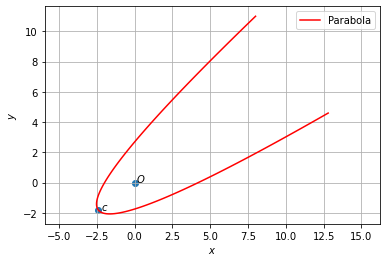
\includegraphics[width=\columnwidth]{./solutions/41/4/assignment5parabola.png}
    \caption{Parabola with vertex c}
    \label{eq:solutions/41/4/fig:fig1}
\end{figure}

%
\item Trace the parabola
\begin{align}\nonumber
    16x^2+24xy+9y^2-5x-10y+1 = 0
\end{align}
%
\solution
Compare the given equation with the standard form
\begin{align}\label{eq:solutions/41/5/eq:1}
    ax^2+2bxy+cy^2+2dx+2ey+f = 0
\end{align}
Write the values Of V and u as follows
\begin{align}
    \vec{V} = \vec{V}^T = \myvec{16 & 12\\12 & 9} \quad
    \vec{u} =\myvec{-\frac{5}{2} \\ -5} \quad
     f = 1 \label{eq:solutions/41/5/eq:2}
\end{align}
The characteristic equation of $\vec{V}$ is given as
\begin{align}
    \mydet{\lambda\vec{I}-\vec{V}} = 0\\
    \implies \mydet{\lambda-16 & -12 \\ -12 & \lambda-9} = 0\\
    \implies \lambda^2 -25\lambda = 0 \label{eq:solutions/41/5/eq:3}
\end{align}
The eigenvalues are the roots of the equation \eqref{eq:solutions/41/5/eq:3} are
\begin{align}
    \lambda_{1} = 0, \quad \lambda_{2} = 25 \label{eq:solutions/41/5/eq:4}
\end{align}
The eigen vector $\vec{p}$ is defined as, 
\begin{align}
    \vec{V}\vec{p} &= \lambda\vec{p}\\
    \implies(\lambda\vec{I}-\vec{V})\vec{p}&=0
\end{align}
For $\lambda_1=0$
\begin{align}
    (\lambda_1\vec{I}-\vec{V}) = \myvec{-16 & -12\\-12 & -9}\xleftrightarrow[R_2\leftarrow R_2-3R_1]{R_1\leftarrow \frac{1}{4}R_1}\myvec{-4 & -3\\0 & 0}
\end{align}
\begin{align}
    \implies\vec{p_1}&=\frac{1}{5}\myvec{-3\\4}\label{eq:solutions/41/5/eq:p1val}
\end{align}
For $\lambda_2=25$
\begin{align}
    (\lambda_2\vec{I}-\vec{V}) = \myvec{9 & -12\\-12 & 16}\xleftrightarrow[R_2\leftarrow R_2+4R_1]{R_1\leftarrow \frac{1}{3}R_1}\myvec{3 & -4\\0 & 0}
\end{align}
\begin{align}
    \implies\vec{p_2}=\frac{1}{5}\myvec{4\\3}\label{eq:solutions/41/5/eq:p2val}
\end{align}
Use Eigenvalue decomposition, $\vec{P}^T\vec{V}\vec{P}=\vec{D}$, where
\begin{align}
    \vec{P} = \frac{1}{5}\myvec{-3 & 4\\4 & 3}\\
    \vec{D} = \myvec{\lambda_1 & 0\\0 & \lambda_2} = \myvec{0 & 0\\ 0 & 25}
\end{align}
Focal length of the parabola is given as
\begin{align}
    \text{focal length} = \abs{\frac{2\eta}{\lambda_2}}\label{eq:solutions/41/5/eq:fl}\\
    \eta = \vec{p}_1^T\vec{u} = -\frac{5}{2}\label{eq:solutions/41/5/eq:eta}\\
    \intertext{Substituting values from \eqref{eq:solutions/41/5/eq:eta} and \eqref{eq:solutions/41/5/eq:4} in \eqref{eq:solutions/41/5/eq:fl}, we get}
    \text{focal length} = \frac{1}{5}
\end{align}
The standard equation of the parabola is given by
\begin{align}
    \vec{y}^T\vec{D}\vec{y} = -2\eta\myvec{1 & 0}\vec{y}
\end{align}
And the vertex $\vec{c}$ is given by
\begin{align}
    \myvec{\vec{u}^T + \eta\vec{p}_1^T \\ \vec{V}}\vec{c} = \myvec{-f \\ \eta\vec{p}_1 - \vec{u}} \label{eq:solutions/41/5/eq:c}
\end{align}
Substituting values from \eqref{eq:solutions/41/5/eq:2},\eqref{eq:solutions/41/5/eq:eta},\eqref{eq:solutions/41/5/eq:p1val} in \eqref{eq:solutions/41/5/eq:c},
\begin{align}
    \myvec{-1 & -7\\16 & 12\\12 & 9}\vec{c} = \myvec{-1\\4\\3}
\end{align}
To find $\vec{c}$, performing row reduction on the augmented matrix as follows:
\begin{align}
    \myvec{-1 & -7 & -1\\16 & 12 & 4\\12 & 9 & 3}\xleftrightarrow[R_1\leftarrow -R_1]{R_3\leftarrow R_3-\frac{3}{4}R_2}\myvec{1 & 7 & 1\\16 & 12 & 4\\0&0&0}\\
    \xleftrightarrow{R_2\leftarrow R_2-16R_1}\myvec{1 & 7 & 1\\0 & -100 & -12\\0&0&0}\\\xleftrightarrow{R_2\leftarrow \frac{-1}{100}R_2}\myvec{1 & 7 & 1\\0 & 1 & \frac{3}{25}\\0&0&0}\\\xleftrightarrow{R_1\leftarrow R_1-7R_2}\myvec{1 & 0 & \frac{4}{25}\\0 & 1 & \frac{3}{25}\\0&0&0}
\end{align}
Thus,
\begin{align}
    \vec{c} = \myvec{\frac{4}{25}\\\frac{3}{25}} %= \myvec{-2.4 \\ -1.8}
\end{align}
\begin{figure}[h!]
    \centering
    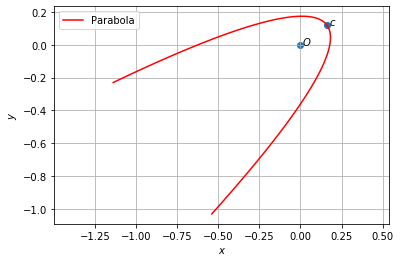
\includegraphics[width=\columnwidth]{./solutions/41/5/A6.png}
    \caption{Parabola with vertex c}
    \label{eq:solutions/41/5/fig:fig1}
\end{figure}

%
\item Trace the parabola
\begin{align}
  9x^2+24xy+16y^2-4y-x+7=0 \label{eq:solutions/41/6/eq:prob}
\end{align}
%
\solution
The general second degree equation can be expressed as
\begin{align}
    \vec{x}^T\vec{V}\vec{x}+2\vec{u}^T\vec{x}+f = 0\label{eq:solutions/41/6/eq:gen}
\end{align}
Comparing \eqref{eq:solutions/41/6/eq:prob} and \eqref{eq:solutions/41/6/eq:gen} we get
\begin{align}
    \vec{V}&=\myvec{9 & 12 \\ 12 & 16}\label{eq:solutions/41/6/eq:V}\\
    \vec{u}&=\myvec{\frac{-1}{2} \\ -2}\label{eq:solutions/41/6/eq:u}\\
    f&=7\label{eq:solutions/41/6/eq:f}
\end{align}
The characteristic equation of $\vec{V}$ is given as
\begin{align}
    \mydet{\vec{V}-\lambda\vec{I}}&=0\\
    \implies\mydet{9-\lambda & 12\\12&16-\lambda}&=0\\
    \implies\lambda^2-25\lambda&=0\label{eq:solutions/41/6/eq:characteristic}
\end{align}
The roots of $\eqref{eq:solutions/41/6/eq:characteristic}$ are eigenvalue of $\vec{V}$ and are given by
\begin{align*}
    \lambda_1=0,\lambda_2=25
\end{align*}
The eigenvector $\vec{p}$ is defined as
\begin{align}
    \vec{V}\vec{p}&=\lambda\vec{p}\\
    \implies(\vec{V}-\lambda\vec{I})\vec{p}&=0\label{eq:solutions/41/6/eq:eigenval}
\end{align}
For $\lambda_1=0$
\begin{align}
    &(\vec{V}-\lambda\vec{I})=\myvec{9&12\\12&16}\xleftrightarrow{R_2=R_2-\frac{4}{3}R_1}\myvec{9&12\\0&0}\label{eq:solutions/41/6/eq:lambda1}
\end{align}
Substituting equation \eqref{eq:solutions/41/6/eq:lambda1} in equation \eqref{eq:solutions/41/6/eq:eigenval} and upon normalization we get
\begin{align}
    \vec{p_1} = \frac{1}{5}\myvec{-4\\3}\label{eq:solutions/41/6/eq:p1}
\end{align}
For $\lambda_2=25$
\begin{align}
    &(\vec{V}-\lambda\vec{I})=\myvec{-16&12\\12&-9}\xleftrightarrow{R_2=R_2+\frac{3}{4}R_1}\myvec{-16&12\\0&0}\label{eq:solutions/41/6/eq:lambda2}
\end{align}
Substituting equation \eqref{eq:solutions/41/6/eq:lambda2} in equation \eqref{eq:solutions/41/6/eq:eigenval} and upon normalization we get
\begin{align}
    \vec{p_2} = \frac{1}{5}\myvec{3\\4}
\end{align}
The matrix $\vec{P}$ and $\vec{D}$ are
\begin{align}
    \vec{P} = \myvec{\vec{p1}&\vec{p2}}=\frac{1}{5}\myvec{-4&3\\3&4}
\end{align}
and
\begin{align}
    \vec{D} = \myvec{\lambda_1&0\\0&\lambda_2} = \myvec{0&0\\0&25}
\end{align}
Then for the parabola
\begin{align}
    \eta = 2\vec{p_1}^T\vec{u}&=-\frac{8}{5}\label{eq:solutions/41/6/eq:eta}\\
    focal\;length =\mydet{\frac{\eta}{\lambda_2}}&=\frac{8}{125}
\end{align}
For parabola $\mydet{\vec{V}}$ = 0,so equation \eqref{eq:solutions/41/6/eq:gen} can be written as
\begin{align}
    \vec{y}^T\vec{D}\vec{y}=-\eta\myvec{1&0}\vec{y}
\end{align}
And the vertex $\vec{c}$ is given by
\begin{align}
    \myvec{\vec{u}^T+\frac{\eta}{2}\vec{p_1}^T\\\vec{V}}\vec{c}=\myvec{-f\\\frac{\eta}{2}\vec{p_1}-\vec{u}}\label{eq:solutions/41/6/eq:c}
\end{align}
Substituting values from \eqref{eq:solutions/41/6/eq:V}, \eqref{eq:solutions/41/6/eq:u}, \eqref{eq:solutions/41/6/eq:f}, \eqref{eq:solutions/41/6/eq:p1}, \eqref{eq:solutions/41/6/eq:eta} in \eqref{eq:solutions/41/6/eq:c}
\begin{align}
    \myvec{\frac{7}{50}&-\frac{124}{50}\\9&12\\12&16}\vec{c}=\myvec{-7\\\frac{57}{50}\\\frac{76}{50}}
\end{align}
To find $\vec{c}$,performing row reduction in augmented matrix as follows
\begin{align*}
    \myvec{\frac{7}{50}&-\frac{124}{50}&-7\\9&12&\frac{57}{50}\\12&16&\frac{76}{50}}\xleftrightarrow[R_1\leftarrow \frac{50}{7}R_1]{R_3\leftarrow R_3-\frac{4}{3}R_2}\myvec{1&-\frac{124}{7}&-50\\9&12&\frac{57}{50}\\0&0&0}\\
    \xleftrightarrow{R_2\leftarrow R_2-9R_1}\myvec{1&-\frac{124}{7}&-50\\0&\frac{1200}{7}&\frac{22557}{50}\\0&0&0}\\
    \xleftrightarrow{R_2\leftarrow\frac{7}{1200}R_2}\myvec{1&-\frac{124}{7}&-50\\0&1&\frac{52633}{20000}\\0&0&0}\\
    \xleftrightarrow{R_1\leftarrow R_1+\frac{124}{7}R_2}\myvec{1&0&-\frac{16911}{5000}\\0&1&\frac{52633}{20000}\\0&0&0}
\end{align*}
Thus
\begin{align}
    \vec{c} = \myvec{-\frac{16911}{5000}\\\frac{52633}{20000}}
\end{align}
  \begin{figure}[!ht]
        \centering
        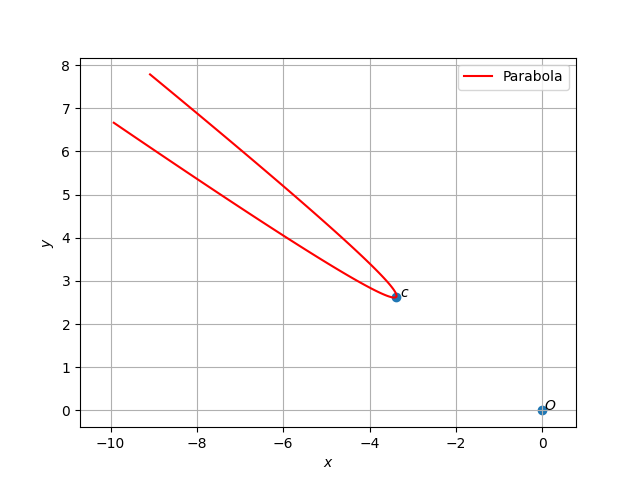
\includegraphics[width=\columnwidth]{./solutions/41/6/parab.png}
        \caption{Graph of $9x^2+24xy+16y^2-4y-x+7=0$}
        \label{eq:solutions/41/6/myfig}
\end{figure}

%
\item Trace the parabola and find its focus.
\begin{align}
144y^2-120xy+25x^2+619x-272y+663=0
\end{align}
%
%
\solution
The general second degree equation can be expressed as follows,
\begin{align}
\Vec{x}^T\Vec{V}\Vec{x}+2\Vec{u}^T\Vec{x}+f=0
\intertext{where,}
\vec{V} &= \myvec{144&-60\\-60&25}\\ \label{eq:solutions/41/7/eq:conics/ex/solution/given1}
\vec{u} &= \myvec{\cfrac{619}{2}\\-136}\\ 
f &= 663 \label{eq:solutions/41/7/eq:conics/ex/solution/given2}
\end{align}
\begin{enumerate}
\item Expanding the determinant of $\vec{V}$ we observe, 
\begin{align}
\mydet{144&-60\\-60&25} = 0 \label{eq:solutions/41/7/eq:conics/ex/solution/eq2.1}
\end{align}
Also
\begin{align}
    \mydet{\vec{V} & \vec{u} \\ \vec{u}^T & f}=
    \mydet{144&-60 & \cfrac{619}{2} \\-60&25 & -136 \\ \cfrac{619}{2} & -136 & 663} \\
    \neq 0\label{eq:solutions/41/7/eq:conics/ex/solution/eq2.2}
\end{align}
Hence from \eqref{eq:solutions/41/7/eq:conics/ex/solution/eq2.1} and \eqref{eq:solutions/41/7/eq:conics/ex/solution/eq2.2} we conclude that given equation is an parabola. The characteristic equation of $\vec{V}$ is given as follows,
\begin{align}
\mydet{\lambda\vec{I}-\vec{V}} = \mydet{\lambda-144&60\\60&\lambda-25} &= 0\\
\implies \lambda^2-169\lambda &= 0\label{eq:solutions/41/7/eq:conics/ex/solution/eqchar}
\end{align}
Hence the characteristic equation of $\vec{V}$ is given by \eqref{eq:solutions/41/7/eq:conics/ex/solution/eqchar}. The roots of \eqref{eq:solutions/41/7/eq:conics/ex/solution/eqchar} i.e the eigenvalues are given by
\begin{align}
\lambda_1=0, \lambda_2=169\label{eq:solutions/41/7/eq:conics/ex/solution/eqeigenvals}    
\end{align}
\item For $\lambda_1 = 0$, the eigen vector $\vec{p}$ is given by 
\begin{align}
\vec{V}\vec{p} = 0
\end{align}
Row reducing $\vec{V}$ yields
\begin{align}
\implies
\myvec{-144&60\\60&-25}\xleftrightarrow[R_2=R_2+5R_1]{R_1=\frac{R_1}{12}}\myvec{-12&5\\0&0}\\
\implies\vec{p}_1=\cfrac{1}{13}\myvec{5\\12} \label{eq:solutions/41/7/eq:conics/ex/solution/eq2.3}
\end{align}
Similarly, 
\begin{align}
\vec{p}_2=\frac{1}{13}\myvec{12\\-5} 
\end{align}
%
Thus, the eigenvector rotation matrix and the eigenvalue matrix are
\begin{align}
\vec{P}&=\myvec{\vec{p_1}&\vec{p_2}}=\frac{1}{13}\myvec{5&12\\ 12 &-5} \\
\vec{D}&=\myvec{0&0\\0&169}
\end{align}
The focal length of the parabola is given by 
\begin{align}
\frac{\abs{2\vec{u}^T\vec{p_1}}}{\lambda_2}
    = \frac{13}{169}=\cfrac{1}{13}
\end{align}
and its equation is
\begin{align}
    \vec{y^T}\vec{D}\vec{y}&=-\eta\myvec{1&0}\vec{y}\label{eq:solutions/41/7/eq:conics/ex/solution/eq2.4}
\end{align}
where
\begin{align}
    \eta=2\vec{u}^T\vec{p_1}=-13
\end{align}
and the vertex $\vec{c}$ is given by 
\begin{align}
    \myvec{\vec{u^T}+\frac{\eta}{2}\vec{p_1^T} \\ \vec{V}}\vec{c}=
    \myvec{-f \\\frac{\eta}{2}\vec{p_1}-\vec{u}} 
\end{align}
using equations \eqref{eq:solutions/41/7/eq:conics/ex/solution/given1},\eqref{eq:solutions/41/7/eq:conics/ex/solution/given2} and \eqref{eq:solutions/41/7/eq:conics/ex/solution/eq2.3}
\begin{align}
    \myvec{307& -142 \\ 144 & -60 \\  -60 & 25 }\vec{c}=\myvec{-663 \\ -312\\ 130} \label{eq:solutions/41/7/eq:conics/ex/solution/eqcen}
\end{align}
Forming the augmented matrix and row reducing it:
\begin{align}
\myvec{307 & -142 & -663\\144 & -60 & -312 \\-60 & 25 &130 }\\
R_2\leftrightarrow \cfrac{R_2}{12} \nonumber \\
\myvec{307 & -142 & -663\\12 & -5 & -26 \\-60 & 25 &130}\\
R_3\leftrightarrow R_3+5R_2 \nonumber \\
\myvec{307 & -142 & -663\\12 & -5 & -26 \\0 & 0 &0}\\
R_1\leftrightarrow \cfrac{R_1}{307} \nonumber \\
\myvec{1 & \cfrac{-142}{307} & \cfrac{-663}{307}\\0 & \cfrac{169}{307} & \cfrac{-26}{307} \\0 & 0 &0}\\ R_2\leftrightarrow R_2-12R_1 \nonumber \\
\myvec{1 & \cfrac{-142}{307} & \cfrac{-663}{307}\\0 & 1 & \cfrac{-26}{307} \\0 & 0 &0}\\
R_1\leftrightarrow R_1 +(142/307)R_2 \nonumber \\
\myvec{1 & 0 & -29/13\\0 & 1 & -2/13 \\0 & 0 &0}
\end{align}
Thus the vertex $\vec{c}$ is:
\begin{align}
\vec{c}=\myvec{ -29/13\\-2/13} 
\end{align}

The direction vector of axis of symmetry is given by :
\begin{align}
\vec{m}=\vec{Vc}+\vec{u}\\
=\myvec{144&-60\\-60&25}\myvec{-\cfrac{29}{13}\\-\cfrac{2}{13}}+\myvec{\cfrac{619}{2}\\-\cfrac{272}{2}}\\
=\myvec{-\cfrac{5}{2}\\-6}\\
\vec{m}=\cfrac{13}{2}\\
\implies \cfrac{\vec{m}}{\norm{\vec{m}}}=\myvec{-\cfrac{5}{13}\\-\cfrac{12}{13}}
\end{align}

The focus is given by:
\begin{align}
\vec{F}=\vec{c}-
\brak{
\frac
{
\vec{m}
}
{
\norm
{
\vec{m}
}
\times a
}
}
\\
=\myvec
{
-\cfrac{29}{13}
\\
-\cfrac{2}{13}
}
-\myvec
{
\myvec
{
-\cfrac{5}{13}
\\
-\cfrac{12}{13}
}
}
\times \cfrac{1}{52}\\
=\myvec{
-\cfrac{1503}{676}
\\
-\cfrac{23}{169}
}
\end{align}

\begin{figure}[!ht]
    \centering
    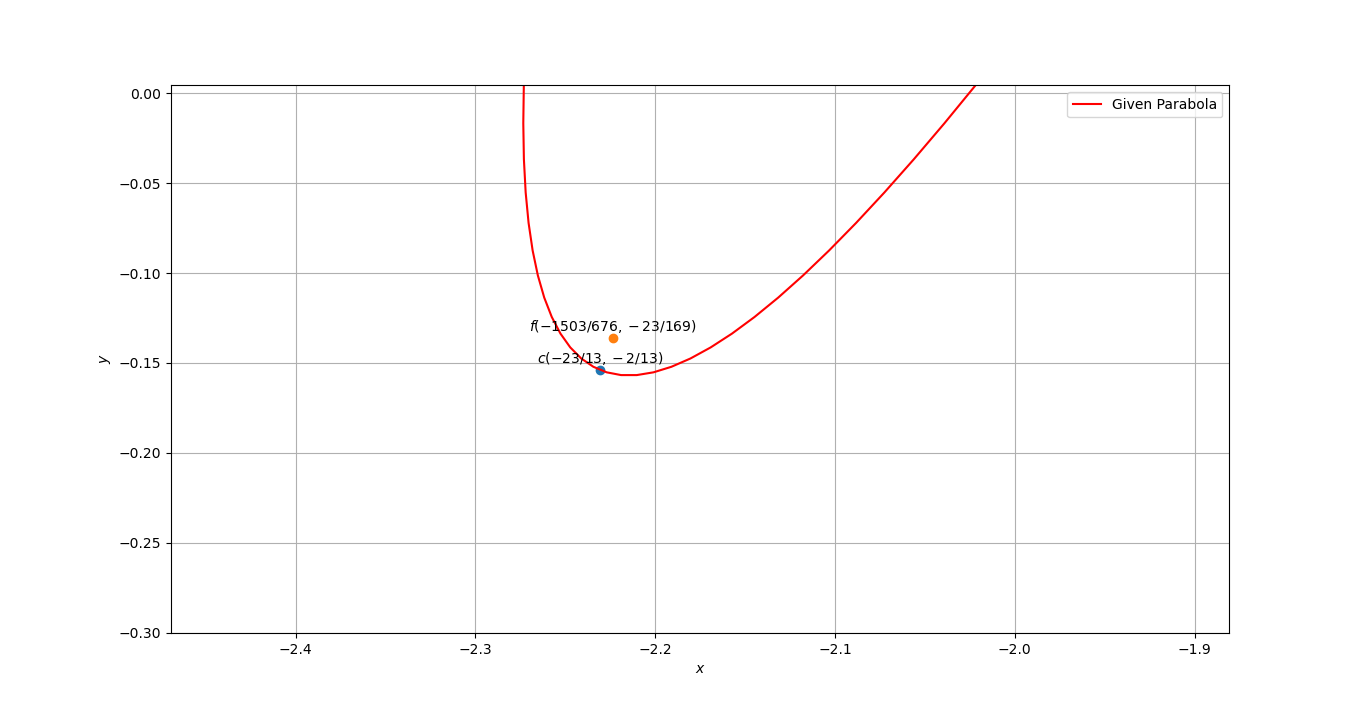
\includegraphics[width=\columnwidth]{./solutions/41/7/figs/parabola}
\caption{Traced parabola}
\label{eq:solutions/41/7/parabola}
\end{figure}

\end{enumerate}




\item Trace the parabola
\begin{align}
   16x^2-24xy+9y^2+32x+86y-39=0 \label{eq:solutions/41/8/eq:given}
\end{align}
%
\solution
The general equation of a second degree can be expressed as: 
\begin{align}
   \vec{x}^T\vec{V}\vec{x}+2\vec{u}^T\vec{x}+f=0 \label{eq:solutions/41/8/eq:conic}
\end{align}
Comparing \eqref{eq:solutions/41/8/eq:given} and \eqref{eq:solutions/41/8/eq:conic}
\begin{align}
\vec{V}=\vec{V}^T =\myvec{16 & -12 \\ -12 & 9 }, \quad\vec{u}=\myvec{16 \\ 43},\quad f=-39 \label{eq:solutions/41/8/eq:parametrics}
\end{align}
{Eigen Values:}
The characteristic equation of $\vec{V}$ is given as
\begin{align}
\mydet{\lambda \vec{I}-\vec{V}} = 0
\end{align}
\begin{align}
\implies \mydet{\lambda-16 & 12 \\ 12 & \lambda-9} =0
\end{align}
\begin{align}
\implies \lambda^2-25\lambda=0 \label{eq:solutions/41/8/eq:chartistic}
\end{align}
The eigenvalues are the roots of the equation \eqref{eq:solutions/41/8/eq:chartistic}, which are as follows:
\begin{align}
 \lambda_1=0, \quad  \lambda_2=25 \label{eq:solutions/41/8/eq:eigenval}
\end{align}
{Eigen Vectors:}
The eigen vector $\vec{p}$ is defined as
\begin{align}
\vec{V}\vec{p}=\lambda\vec{p}     
\end{align}
\begin{align}
\implies (\lambda \vec{I} - \vec{V} ) \vec{p} = 0
\end{align}
For $\lambda_1 = 0 $
\begin{align}
(\lambda_1 \vec{I}-\vec{V} ) = \myvec{-16 & 12 \\ 12 & -9 }\xleftrightarrow[R_2\leftarrow R_2+3R_1]{R_1\leftarrow \frac{1}{4}R_1}\myvec{-4 & 3\\0 & 0}
\end{align}
\begin{align}
\implies \vec{p_1} = \frac{1}{5} \myvec{3 \\ 4} \label{eq:solutions/41/8/eq:p1val}
\end{align}
For $\lambda_2 = 25$
\begin{align}
(\lambda_2 \vec{I}-\vec{V} ) = \myvec{9 & 12 \\ 12 & 1}\xleftrightarrow[R_2\leftarrow R_2-4R_1]{R_1\leftarrow \frac{1}{3}R_1}\myvec{3 & 4\\0 & 0}
\end{align}
\begin{align}
\implies \vec{p_2} = \frac{1}{5} \myvec{-4\\ 3} \label{eq:solutions/41/8/eq:p2val}
\end{align}
{Eigen Value Decomposition:}
Using EVD, we can write 
\begin{align}
 \vec{D} = \vec{P} \vec{V} \vec{P}^T
\end{align}
From \eqref{eq:solutions/41/8/eq:p1val} and \eqref{eq:solutions/41/8/eq:p2val}
\begin{align}
 \vec{P} = \frac{1}{5} \myvec{3 & -4 \\ 4 & 3}
\end{align}
From \eqref{eq:solutions/41/8/eq:eigenval}
\begin{align}
 \vec{D} = \myvec{\lambda_1 & 0 \\ 0 & \lambda_2} = \myvec{0 & 0 \\ 0 & 25}
\end{align}
{Parabola}
\begin{align}
\text{Focal Length} = \abs{\frac{2\eta}{\lambda_2}} \label{eq:solutions/41/8/eq:focallen}\\
\intertext{From \eqref{eq:solutions/41/8/eq:p1val} and \eqref{eq:solutions/41/8/eq:parametrics}}
\eta = \vec{p}_1^T\vec{u} = 44 \label{eq:solutions/41/8/eq:etaval}\\
\intertext{Substituting values of \eqref{eq:solutions/41/8/eq:etaval} and \eqref{eq:solutions/41/8/eq:eigenval} in \eqref{eq:solutions/41/8/eq:focallen}, we get}
\text{Focal Length} = \abs{\frac{88}{25}}=3.52
\end{align}
The standard equation of parabola is given by:
\begin{align}
 \vec{y}^T\vec{D}\vec{y} = -2\eta \myvec{1 & 0}\vec{y} \label{eq:solutions/41/8/eq:parabola}
\end{align}
And the vertex $\vec{c}$ is:
\begin{align}
 \myvec{\vec{u}^T+\eta \vec{p_1}^T \\ \vec{V}}\vec{c} = \myvec{-f \\ \eta \vec{p_1}-\vec{u}}
\end{align}
From \eqref{eq:solutions/41/8/eq:parametrics} \eqref{eq:solutions/41/8/eq:etaval} and \eqref{eq:solutions/41/8/eq:p1val},
\begin{align}
\myvec{\frac{212}{5} & \frac{391}{5} \\ 16 & -12 \\ -12 & 9}\vec{c}=\myvec{39 \\ \frac{52}{5}\\ \frac{-39}{5}}
\end{align}
To find $\vec{c}$, perform row reduction on the augmented matrix as follows:
\begin{align}
    \myvec{\frac{212}{5} & \frac{391}{5} & 39\\16 & -12 & \frac{52}{5}\\-12 & 9 & \frac{-39}{5}}\xleftrightarrow[R_1\leftarrow \frac{5}{212}R_1]{R_3\leftarrow R_3+\frac{3}{4}R_2}\myvec{1 & \frac{391}{212} & \frac{195}{212}\\16 & -12 & \frac{52}{5}\\0&0&0}\\
    \xleftrightarrow{R_2\leftarrow R_2-16R_1}\myvec{ 1 & \frac{391}{212} & \frac{195}{212}\\0 & \frac{-2200}{53} & \frac{-1144}{265} \\0&0&0}\\\xleftrightarrow{R_2\leftarrow \frac{-53}{2200}R_2}\myvec{1 & \frac{391}{212} & \frac{195}{212} \\0 & 1 & \frac{13}{125}\\0&0&0}\\\xleftrightarrow{R_1\leftarrow R_1-\frac{391}{212}R_2}\myvec{1 & 0 & \frac{4823}{6625}\\0 & 1 & \frac{13}{125}\\0&0&0}
\end{align}
Hence,
\begin{align}
\vec{c}=\myvec{\frac{4823}{6625}\\ \frac{13}{125}}= \myvec{0.728 \\ 0.104}
\end{align}
\begin{figure}[h!]
	\centering
	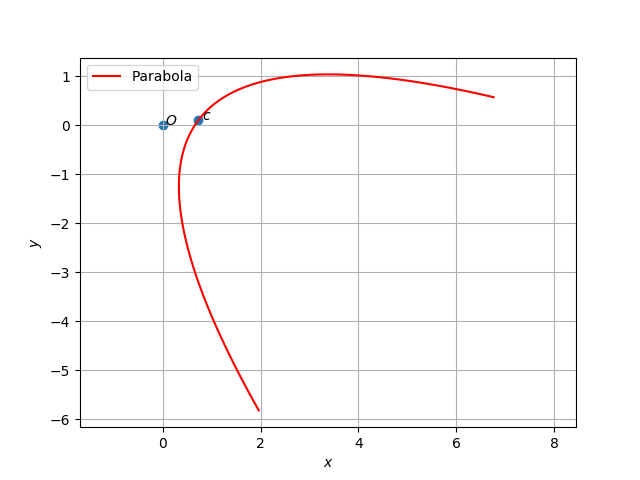
\includegraphics[width=\columnwidth]{./solutions/41/8/Codes/A5.png}
	\caption{Parabola with vertex c }
	\label{eq:solutions/41/8/myfig}
\end{figure}

\item Trace the following parabola
\begin{align}
    4x^2-4xy+y^2-12x+6y+9=0
\end{align}
%
%
\solution
The given quadratic equation can be written in the matrix form as
\begin{align}
    \vec{x}^T\myvec{4&-2\\-2&1}\vec{x}+2\myvec{-6&3}\vec{x}+9=0\label{eq:solutions/41/9/eq:1}
\end{align}
Calculating the parameters,we get
\begin{align}
    \mydet{\vec{V}}=\mydet{4&-2\\-2&1}=0\\
    \mydet{\vec{V}&\vec{u}\\\vec{u}^T&f}=\mydet{4&-2&-6\\-2&1&3\\-6&3&9}=0
\end{align}
Therefore the given parabola equation is a degenerate.The quadratic equation corresponds to a pair of coincident straight lines.\par
The characteristic equation of $\vec{V}$ will be
\begin{align}
    \mydet{\vec{V}-\lambda\vec{I}}&=\mydet{4-\lambda&-2\\-2&1-\lambda}\\
    &=\lambda^2-5\lambda\\
    &\lambda_1=0,\lambda_2=5
\end{align}
The eigen vectors are the nullspace of the matrix $\vec{V}-\lambda\vec{I}$.For $\lambda_1=0$
\begin{align}
    \myvec{4&-2\\-2&1}\xleftrightarrow{R_2=2R_2+R_1}\myvec{4&-2\\0&0}\\
    p_1=\myvec{1\\2}
\end{align}
Therefore the normalized eigen vector will be
\begin{align}
    p_1=\myvec{\frac{1}{\sqrt{5}}\\\frac{2}{\sqrt{5}}}
\end{align}
For $\lambda_2=5$
\begin{align}
    \myvec{-1&-2\\-2&-4}\xleftrightarrow{R_2=R_2-2R_1}\myvec{-1&-2\\0&0}\\
    p_2=\myvec{-2\\1}
\end{align}
Therefore the normalized eigen vector will be
\begin{align}
    p_2=\myvec{-\frac{2}{\sqrt{5}}\\\frac{1}{\sqrt{5}}}
\end{align}
Therefore the transformation matrix will be
\begin{align}
    \vec{P}=\myvec{p_1&p_2}=\myvec{\frac{1}{\sqrt{5}}&-\frac{2}{\sqrt{5}}\\\frac{2}{\sqrt{5}}&\frac{1}{\sqrt{5}}}
\end{align}
The value of $\eta$ will be
\begin{align}
    \eta&=2p_1^T\vec{u}\\
    &=2\myvec{\frac{1}{\sqrt{5}}&\frac{2}{\sqrt{5}}}\myvec{-6\\3}\\
    &=0
\end{align}
A point on the line can be found by using to following formula
\begin{align}
    \myvec{\vec{u}^T+\frac{\eta}{2}p_1^T\\\vec{V}}c=\myvec{-f\\\frac{\eta}{2}p_1-\vec{u}}\\
    \myvec{\vec{u}^T\\\vec{V}}c=\myvec{-f\\-\vec{u}}\\
    \myvec{-6&3\\4&-2\\-2&1}c=\myvec{-9\\6\\-3}
\end{align}
Writing it in augmented form, we get
\begin{align}
    \myvec{-6&3&-9\\4&-2&6\\-2&1&-3}\xleftrightarrow{R_3=R_3-\frac{R_1}{3}}\myvec{-6&3&-9\\4&-2&6\\0&0&0}\\
    \xleftrightarrow{R_2=\frac{3}{2}R_2+R_1}\myvec{-6&3&-9\\0&0&0\\0&0&0}
\end{align}
Therefore we can see that the point $c=\myvec{1\\-1}$ lies on the line.
{Equation of the straight line}
Applying affine transformation we get
\begin{align}
    \vec{y}^T\vec{D}\vec{y}=-\eta\myvec{1&0}\vec{y}\\
    \vec{y}^T\myvec{0&0\\0&5}\vec{y}=0\\
    5y^2=0
\end{align}
Therefore the transformed line is $y=0$,which in vector form will be $\myvec{0&1}\vec{y}=0$.\par
Taking the Inverse affine transformation we get
\begin{align}
    \myvec{0&1}\brak{P^T\brak{\vec{x}-c}}=0\\
    \myvec{0&1}\myvec{\frac{1}{\sqrt{5}}&\frac{2}{\sqrt{5}}\\-\frac{2}{\sqrt{5}}&\frac{1}{\sqrt{5}}}\brak{\vec{x}-c}=0\\
    \myvec{-\frac{2}{\sqrt{5}}&\frac{1}{\sqrt{5}}}\brak{\vec{x}-c}=0\\
    \myvec{-\frac{2}{\sqrt{5}}&\frac{1}{\sqrt{5}}}\vec{x}-\myvec{-\frac{2}{\sqrt{5}}&\frac{1}{\sqrt{5}}}\myvec{1\\-1}=0\\
    \myvec{-\frac{2}{\sqrt{5}}&\frac{1}{\sqrt{5}}}\vec{x}+\frac{3}{\sqrt{5}}=0\\
    \myvec{2&-1}\vec{x}=3
\end{align}
Therefore the equation of coincident lines is $\brak{2x-y-3}=0$.

%
\item Trace the central conic,
\begin{align}
2x^2 - 2xy + y^2 + 2x - 2y = 0\label{eq:solutions/41/17/eq:1}
\end{align}
%
\\
\solution
The general equation of a second degree (In algebraic form) can be expressed as,
\begin{align}
ax^2 + 2bxy + cy^2 + 2dx + 2ey + f = 0 \label{eq:solutions/41/17/eq:2}
\end{align}
The general equation of a second degree (In vector form) can be expressed as,
\begin{align}
\vec{x^T}\vec{V}\vec{x} + 2\vec{u^T}\vec{x} + f = 0
\end{align}
Comparing \eqref{eq:solutions/41/17/eq:1} with \eqref{eq:solutions/41/17/eq:2} , we get,
\begin{align}
a = 2, \ b = -1, \ c = 1, \ d = 1, \ e = -1 \ and \ f = 0
\end{align}
where,
\begin{align}
\vec{V} = \myvec{a & b \\ b & c} = \myvec{2 & -1 \\ -1 & 1} = \vec{V^T}\\
\implies \vec{V} = \myvec{2 & -1 \\ -1 & 1}
\end{align}
and
\begin{align}
\vec{u} = \myvec{1 \\ -1}    
\end{align}
Finding the determinant of V we obtain, 
\begin{align}
|\vec{V}| = 1 > 0
\end{align}
which means the given central conic is an ellipse which can be proven more effectively using,
\begin{align}
\vec{V} = \vec{PDP^T}\label{eq:solutions/41/17/eq:9}    
\end{align}
where $\vec{P}$ is a matrix of Eigen vectors and $\vec{D}$ is a diagonal matrix of Eigen values which will be computed subsequently.\\
Computing Eigen values for $\vec{V}$ using the characteristic equation of the matrix, we get the following quadratic equation in terms of $\lambda$
\begin{align}
\lambda^{2} - 3\lambda + 1 = 0\\
\implies \lambda_{1} = \frac{3 + \sqrt{5}}{2} \ and \ \lambda_{2} = \frac{3 - \sqrt{5}}{2}
\end{align}
Eigen vectors can be computed using the following equation,
\begin{align}
(\lambda\vec{I - V})\vec{p} = 0
\end{align}
Solving this for $\lambda_{1}$ and $\lambda_{2}$ respectively and normalizing them we obtain,
\begin{align}
\vec{p_1} = \sqrt{\frac{2}{5-\sqrt{5}}}\myvec{1 \\[1em] \frac{1-\sqrt{5}}{2}}\\
\vec{p_2} = \sqrt{\frac{2}{5+\sqrt{5}}}\myvec{1 \\[1em] \frac{\sqrt{5}+1}{2}}
\end{align}
Simplifying, 
\begin{align}
\implies \vec{P} = \myvec{\sqrt{\frac{2}{5-\sqrt{5}}} & \sqrt{\frac{2}{5+\sqrt{5}}} \\[1em] \frac{1-\sqrt{5}}{\sqrt{5\sqrt{2}-\sqrt{10}}} & \frac{1+\sqrt{5}}{\sqrt{5\sqrt{2}+\sqrt{10}}}} \label{eq:solutions/41/17/eq:15}
\end{align}
\begin{align}
\vec{D} = \myvec{\frac{3+\sqrt{5}}{2} & 0 \\ 0 & \frac{3-\sqrt{5}}{2}}
\end{align}
Using \eqref{eq:solutions/41/17/eq:9} can verify that it holds which means that the given central conic is an ellipse.
The center of the ellipse can be computed using,
\begin{align}
\vec{c} = \vec{-V^{-1}u}\\
\implies \vec{c} = \myvec{0 \\ 1} \label{eq:solutions/41/17/eq:18}
\end{align}
The parameters of the ellipse are computed as follows,
\begin{align}
\sqrt{\frac{{\vec{u^{T}V^{-1}u} - f}}{\lambda_{1}}} = \sqrt{\frac{3-\sqrt{5}}{2}}\\
\sqrt{\frac{{\vec{u^{T}V^{-1}u} - f}}{\lambda_{2}}} = \sqrt{\frac{3+\sqrt{5}}{2}}
\end{align}
The angle of Rotation can be obtained by equating $\vec{P}$ with the Rotation matrix which is,
\begin{align}
\vec{P} = \myvec{\cos{\theta} & \sin{\theta} \\ -\sin{\theta} & cos{\theta}} \label{eq:solutions/41/17/eq:21}
\end{align}
Comparing \eqref{eq:solutions/41/17/eq:15} and \eqref{eq:solutions/41/17/eq:21} we get,
\begin{align}
\theta = \frac{\pi}{5.66} \label{eq:solutions/41/17/eq:22}  
\end{align}
Using the Affine transformation we find out the actual ellipse,
\begin{align}
\vec{y} = \vec{P^Tx} + \vec{c}     
\end{align}
which means the actual ellipse is obtained by translating and rotating the standard ellipse w.r.t center, $\vec{c}$ from \eqref{eq:solutions/41/17/eq:18} and angle of rotation, $\theta$ from \eqref{eq:solutions/41/17/eq:22} respectively.\\
Using the above data along with $\vec{o}$ (Origin), the center of the standard ellipse, the actual ellipse is plotted as follows.  
\begin{figure}[!ht]
    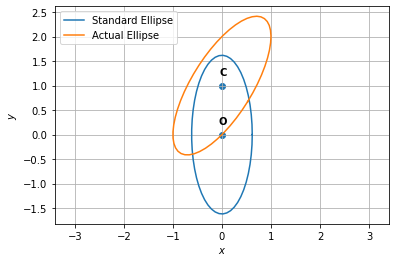
\includegraphics[width=\columnwidth]{solutions/41/17/Figure.png}
    \caption{Standard and Actual Ellipses}
    \label{eq:solutions/41/17/Fig.1}
\end{figure}

\item Trace the following central conic : 
\begin{align}
    x^2+y^2+xy+x+y=1\label{eq:solutions/41/18/eq:0}
\end{align}
%
\\
\solution
General equation of second degree is given by :
\begin{align}
\vec{x}^T\vec{V}\vec{x}+2\vec{u}^T\vec{x}+f=0\label{eq:solutions/41/18/eq:1}
\end{align}
In the vector form \eqref{eq:solutions/41/18/eq:0} can be written as :
\begin{align}
\vec{x}^T\myvec{1&\frac{1}{2}\\[0.1cm]\frac{1}{2}&1}\vec{x}+2\myvec{\frac{1}{2}\\[0.1 cm]\frac{1}{2}}^T\vec{x}-1=0\label{eq:solutions/41/18/eq:2}
\end{align}
By comparing \eqref{eq:solutions/41/18/eq:1} and \eqref{eq:solutions/41/18/eq:2} we get : 
\begin{align}
    \vec{V}=\myvec{1&\frac{1}{2}\\[0.1cm]\frac{1}{2}&1},\vec{u}=\myvec{\frac{1}{2}\\[0.1 cm]\frac{1}{2}},f=-1\label{eq:solutions/41/18/eq:3}
\end{align}
Eigen values for matrix $\vec{V}$ can be calculated by solving :  
\begin{align}
    \mydet{1-\lambda&\frac{1}{2}\\[0.1cm]\frac{1}{2}&1-\lambda}&=0\\
    \lambda^2-2\lambda+\frac{3}{4}&=0\\
    \lambda_1=\frac{3}{2},\lambda_2&=\frac{1}{2}
\end{align}
By doing Eigenvalue Decomposition and Affine Transformation we get : 
\begin{align}
    \vec{P}^{-1}\vec{V}\vec{P}&=\vec{D}=\myvec{\lambda_1&0\\0&\lambda_2}\\
    \vec{x}&=\vec{P}\vec{y}+\vec{c}\label{eq:solutions/41/18/eq:8}
\end{align}
Where the matrix $\vec{P}$ is normalised eigenbasis and $\vec{c}$ is the center.\\
By putting the value of $\vec{x}$ from \eqref{eq:solutions/41/18/eq:8} in \eqref{eq:solutions/41/18/eq:1} we get : 
\begin{align}
    (\vec{P}\vec{y}+\vec{c})^T\vec{V}(\vec{P}\vec{y}+\vec{c})+2\vec{u}^T\vec{x}+f=0
\end{align}
Further solving this we get : 
\begin{align}
    \vec{V}\vec{c}+\vec{u}&=0\implies\vec{c}=-\vec{V}^{-1}\vec{u}\label{eq:solutions/41/18/eq:10}\\
    \vec{y}^T\vec{D}\vec{y}&=\vec{u}^T\vec{V}^{-1}\vec{u}-f\label{eq:solutions/41/18/eq:11}
\end{align}
As
\begin{align}
    \mydet{\vec{V}} =\mydet{1&\frac{1}{2}\\[0.1cm]\frac{1}{2}&1}=\frac{3}{4}>0
\end{align}
Equation \eqref{eq:solutions/41/18/eq:11} forms an ellipse centered at origin with major and minor axis given as : 
\begin{align}
    a=\sqrt{\frac{\vec{u}^T\vec{V}^{-1}\vec{u}-f}{\lambda_1}}\label{eq:solutions/41/18/eq:13}\\
    b=\sqrt{\frac{\vec{u}^T\vec{V}^{-1}\vec{u}-f}{\lambda_2}}\label{eq:solutions/41/18/eq:14}
\end{align} 
Using Gauss Jordan Elimination on matrix $\vec{V}$ : 
\begin{align}
 \xleftrightarrow{R_2 \leftarrow \frac{1}{2} R_1-R_2}\myvec{1&\frac{1}{2}&:&1&0\\[0.1cm]0&\frac{-3}{4}&:&\frac{1}{2}&-1}\\
 \xleftrightarrow{R_2 \leftarrow \frac{-4}{3} R_2}\myvec{1&\frac{1}{2}&:&1&0\\[0.1cm]0&1&:&\frac{-2}{3}&\frac{4}{3}}\\
 \xleftrightarrow{R_1 \leftarrow R_1-\frac{1}{2} R_2}\myvec{1&0&:&\frac{4}{3}&\frac{-2}{3}\\[0.1cm]0&1&:&\frac{-2}{3}&\frac{4}{3}}
 \end{align}
 Therefore,
 \begin{align}
 \vec{V}^{-1}=\myvec{\frac{4}{3}&\frac{-2}{3}\\[0.2cm]\frac{4}{3}&\frac{-2}{3}}\label{eq:solutions/41/18/eq:18}
\end{align}
Using \eqref{eq:solutions/41/18/eq:10} and \eqref{eq:solutions/41/18/eq:18} we get : 
\begin{align}
    \vec{c}=-\vec{V}^{-1}\vec{u}=-\myvec{\frac{4}{3}&\frac{-2}{3}\\[0.2cm]\frac{4}{3}&\frac{-2}{3}}\myvec{\frac{1}{2}\\[0.2cm]\frac{1}{2}}=\myvec{\frac{-3}{10}\\[0.2cm]\frac{-3}{10}}
\end{align}
By putting the values of $\vec{u}$, $\vec{V}^{-1}$, $f$, $\lambda_1$ and $\lambda_2$ in \eqref{eq:solutions/41/18/eq:13} and \eqref{eq:solutions/41/18/eq:14} respectively we get :   
\begin{align}
    a&=\sqrt{\frac{\myvec{\frac{1}{2}&\frac{1}{2}}\myvec{\frac{4}{3}&\frac{-2}{3}\\[0.2cm]\frac{4}{3}&\frac{-2}{3}}\myvec{\frac{1}{2}\\[0.2cm]\frac{1}{2}}-1}{\frac{3}{2}}}=\frac{9}{10}\\
    b&=\sqrt{\frac{\myvec{\frac{1}{2}&\frac{1}{2}}\myvec{\frac{4}{3}&\frac{-2}{3}\\[0.2cm]\frac{4}{3}&\frac{-2}{3}}\myvec{\frac{1}{2}\\[0.2cm]\frac{1}{2}}-1}{\frac{1}{2}}}=\frac{8}{5}
\end{align}

In the transformed space with Eigenbasis, an ellipse centered at origin with major and minor axis as $a$ and $b$ is traced as 'Standard Ellipse' in the plot.\\


And after doing Affine Transformation on $\vec{y}$ as in \eqref{eq:solutions/41/18/eq:8} we get our 'Actual Ellipse' centered at $\vec{c}$ shown in the plot.
\begin{figure}[h]
\centering
    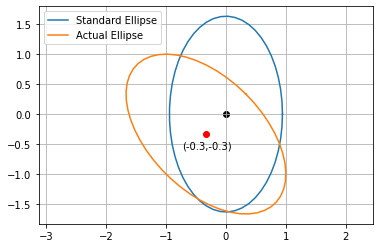
\includegraphics[width=\columnwidth]{solutions/41/18/ellipse.png}
    \caption{Standard Ellipse centered at origin and Actual Ellipse centered at $(-0.3,-0.3)$.}
    \label{eq:solutions/41/18/tangent}
\end{figure}

\item Trace the following central conic:
\begin{align}
  2x^2 + 3xy - 2y^2 - 7x + y - 2 = 0 \label{eq:solutions/41/19/eq:1}
\end{align}
%
\\
\solution
Any second degree equation of the form:
\begin{align}
  ax^2 + 2bxy + cy^2 + 2dx + 2ey + f = 0
\end{align}
Can be represented in matrix / vector form as:
\begin{align}
  \vec{x}^T\vec{Vx} + 2\vec{u}^T\vec{x} + f = 0
\end{align}
where,
\begin{align}
  \vec{V} = \vec{V}^T = \myvec{a & b \\ b & c} \\
  \vec{u} = \myvec{d & e}
\end{align}
Rewriting \eqref{eq:solutions/41/19/eq:1} in matrix form, we get:
\begin{align}
  \vec{x}^T\myvec{2 & \frac{3}{2} \\\frac{3}{2} & -2}\vec{x} + 2\myvec{-\frac{7}{2} & \frac{1}{2}} - 2 = 0
\end{align}
where,
\begin{align}
  \vec{V} = \myvec{2 & \frac{3}{2} \\\frac{3}{2} & -2} \\
  \vec{u} = \myvec{-\frac{7}{2} \\[0.2cm] \frac{1}{2}} \\
  f = -2 \\
  det(\vec{V}) = \mydet{2 & \frac{3}{2} \\\frac{3}{2} & -2} = -\frac{25}{4}
\end{align}
As $det(\vec{V}) < 0$, the given conic represents a hyperbola. \\
The characteristic equation of $\vec{V}$ is given by the determinant:
\begin{align}
  \mydet{\vec{V} - \lambda\vec{I}} = 0 \\
  \mydet{2 - \lambda & \frac{3}{2} \\\frac{3}{2} & -2 - \lambda} = 0 \\
  \implies \lambda^{2} - \frac{25}{4} = 0 \label{eq:solutions/41/19/eq:2}
\end{align}
The roots of \eqref{eq:solutions/41/19/eq:2} (the eigenvalues) are:
\begin{align}
  \lambda_1 = \frac{5}{2}, \lambda_2 = -\frac{5}{2}
\end{align}
The eigenvector $\vec{p}$ is defined as:
\begin{align}
  \vec{Vp} = \lambda \vec{p} \\
  \implies (\vec{V} - \lambda \vec{I})\vec{p} = 0 \label{eq:solutions/41/19/eq:3}
\end{align}
Evaluating \eqref{eq:solutions/41/19/eq:3} for $\lambda_1 = \frac{5}{2}$, we get:
\begin{align}
  (\vec{V} - \lambda_1 \vec{I})  = \myvec{-\frac{1}{2} & \frac{3}{2} \\[0.2cm]\frac{3}{2} & -\frac{9}{2}}
\end{align}
Reducing the above equation to row-echelon form, we get:
\begin{align}
  \xleftrightarrow[]{R_2 \rightarrow R_2 + 3R_1} \myvec{-\frac{1}{2} & \frac{3}{2} \\[0.2cm]0 & 0} \xleftrightarrow[]{R_1 \rightarrow -2R_1} \myvec{1 & -3 \\ 0 & 0} \label{eq:solutions/41/19/eq:4}
\end{align}
Substituting \eqref{eq:solutions/41/19/eq:4} in \eqref{eq:solutions/41/19/eq:3}, we get:
\begin{align}
  \myvec{1 & -3 \\ 0 & 0} \myvec{v_1 \\ v_2} = \myvec{0 \\ 0}
\end{align}
where,
\begin{align}
  \vec{p} = \myvec{v_1 \\ v_2}
\end{align}
Let $v_2 = t$. Then
\begin{align}
  v_1 = 3t
\end{align}
Let $t = 1$. The eigenvector $\vec{p_1}$ is:
\begin{align}
  \vec{p_1} = \myvec{3 \\ 1}
\end{align}
Similarly for $\lambda_2 = -\frac{5}{2}$, we get:
\begin{align}
    (\vec{V} - \lambda_2 \vec{I})  = \myvec{\frac{9}{2} & \frac{3}{2} \\[0.2cm]\frac{3}{2} & \frac{1}{2}} \xleftrightarrow[R_1 \rightarrow \frac{2}{9}R_1]{R_2 \rightarrow 3R_2 - R_1} \myvec{1 & \frac{1}{3} \\[0.2cm]0 & 0} \label{eq:solutions/41/19/eq:5}
\end{align}
Substituting \eqref{eq:solutions/41/19/eq:5} in \eqref{eq:solutions/41/19/eq:3}, we get:
\begin{align}
  \myvec{1 & \frac{1}{3} \\[0.2cm]0 & 0} \myvec{v_1 \\ v_2} = \myvec{0 \\ 0}
\end{align}
where,
\begin{align}
  \vec{p} = \myvec{v_1 \\ v_2}
\end{align}
Let $v_2 = t$. Then
\begin{align}
  v_1 = \frac{-t}{3}
\end{align}
Let $t = 1$. The eigenvector $\vec{p_2}$ is:
\begin{align}
  \vec{p_2} = \myvec{\frac{-1}{3} \\[0.2cm] 1}
\end{align}
As $\vec{V} = \vec{V}^T$, there exists an orthogonal matrix P such that:
\begin{align}
  \vec{PVP}^T = \vec{D} = diag(\lambda_1, \lambda_2)
\end{align}
$\vec{V}$ can be rewritten using the above equation as:
\begin{align}
  \vec{V} = \vec{PDP}^T
\end{align}
where,
\begin{align}
  \vec{P} = \myvec{\vec{p_1} & \vec{p_2}} \\
  \vec{D} = \myvec{\lambda_1 & 0 \\ 0 & \lambda_2}
\end{align}
Substituting the values -
\begin{align}
  \vec{P} = \myvec{3 & \frac{-1}{3}\\[0.2cm] 1 & 1} \\
  \vec{D} = \myvec{\frac{5}{2} & 0 \\[0.2cm] 0 & \frac{-5}{2}}
\end{align}
The center of hyperbola is given by:
\begin{align}
  \vec{c} = -\vec{V}^{-1}\vec{u} \\
  \implies \vec{c} = -\myvec{\frac{8}{25} & \frac{6}{25} \\[0.2cm] \frac{6}{25} & \frac{-8}{25}} \myvec{\frac{-7}{2} \\[0.2cm]\frac{1}{2}} = \myvec{1 \\ 1}
\end{align}
As
\begin{align}
  \vec{u}^T\vec{V}^{-1}\vec{u} - f = 5 > 0
\end{align}
there is no requirement for swapping the axes (which will be evident from the equation below). The axes of the hyperbola are given by:
\begin{align}
  axes = \begin{cases}
    \sqrt[]{\frac{\vec{u}^T\vec{V}^{-1}\vec{u} - f}{\lambda_1}} \\
    \sqrt[]{\frac{f - \vec{u}^T\vec{V}^{-1}\vec{u}}{\lambda_2}}
  \end{cases} \\
  \implies \sqrt[]{\frac{\vec{u}^T\vec{V}^{-1}\vec{u} - f}{\lambda_1}} = \sqrt[]{2} \\
  \implies \sqrt[]{\frac{f - \vec{u}^T\vec{V}^{-1}\vec{u}}{\lambda_2}} = \sqrt[]{2}
\end{align}
The standard form of conic is written as:
\begin{align}
  \vec{y}^T\vec{Dy} = \vec{u}^T\vec{V}^{-1}\vec{u} - f
\end{align}
where,
\begin{align}
  \vec{y} = \vec{P}^T(\vec{x-c}) \\
  \implies \vec{y}^T \myvec{\frac{5}{2} & 0 \\[0.2cm] 0 & \frac{-5}{2}} \vec{y} -5 = 0
\end{align}
The plot of both the conics are given below:
\begin{figure}[h!]
\centering
    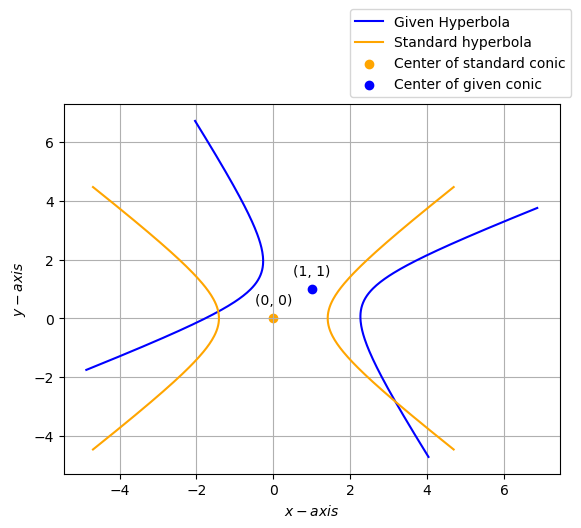
\includegraphics[width=\columnwidth]{solutions/41/19/Latex/hyperbola.png}
    \caption{Plot of given hyperbola and the standard hyperbola}
    \label{eq:solutions/41/19/fig:1}
\end{figure}

\item Trace the following central conics:
\begin{align}
   40{x^2}+36{xy}+25{y^2}-196{x}-122{y}+205=0
\end{align}
%
\\
\solution
The general equation of a second degree can
be expressed as:
\begin{align}
a{x^2}+2b{xy}+c{y^2}+2d{x}+2e{y}+f=0\label{eq:solutions/41/20/geneqn}\\
   \Longrightarrow \vec{x^TVx}+2\vec{u^Tx}+f=0\label{eq:solutions/41/20/geneqn2}
\end{align}
where\begin{align}
\vec{V} =\myvec{a\quad b\\b\quad c},\vec{u}=\myvec{d\\e}\label{eq:solutions/41/20/paraeqn} 
\end{align}
The given equation of the curve can be expressed as:
\begin{align}
    40{x^2}+2(18){xy}+25{y^2}+2(-98){x}+2(-61){y}+205=0\label{eq:solutions/41/20/giveneqn}
\end{align}
Comparing \eqref{eq:solutions/41/20/geneqn},\eqref{eq:solutions/41/20/paraeqn} and \eqref{eq:solutions/41/20/giveneqn}:\\
\begin{align}
\vec{V} = \myvec{40\quad\sqrt{18}\\\sqrt{18}\quad 25},\vec{u}=\myvec{-98\\-61} and\quad f=205 \\
       \Longrightarrow\mydet{\vec{V}}=982\quad and \quad b^2-ac=18-40.25 =-982
\end{align}
Since $\mydet{\vec{V}}>0$\quad and \quad $b^2<ac$ , \eqref{eq:solutions/41/20/giveneqn} represent an ellipse. \\
 The characteristic equation of $\vec{V}$ is given as follows,
\begin{align}
\mydet{\lambda\vec{I}-\vec{V}} = \mydet{\lambda-40\quad\sqrt{18}\\\sqrt{18}\quad\lambda -25} &= 0\\
\implies \lambda^2-65\lambda+982 &= 0\label{eq:solutions/41/20/eqchar}
\end{align}
Hence the characteristic equation of $\vec{V}$ is given by \eqref{eq:solutions/41/20/eqchar}. The roots of \eqref{eq:solutions/41/20/eqchar} i.e the eigenvalues are given by
\begin{align}
\lambda_1=\frac{65+\sqrt{297}}{2}, \lambda_2=\frac{65-\sqrt{297}}{2}\label{eq:solutions/41/20/eqeigenvals}    
\end{align}
The eigen vector $\vec{p}$ is defined as, 
\begin{align}
\vec{V}\vec{p} &= \lambda\vec{p}\\
\implies\brak{\lambda\vec{I}-\vec{V}}\vec{p}&=0\label{eq:solutions/41/20/eqneigvenvec}
\end{align}
for $\lambda_1=\frac{65+\sqrt{297}}{2}$,
\begin{align}
\brak{\lambda_1\vec{I}-\vec{V}}=\myvec{\frac{\sqrt{297}-15}{2}&-\sqrt{18}\\-\sqrt{18}&\frac{\sqrt{297}+15}{2}}\\\xleftrightarrow{R_2=R_2+\frac{2\sqrt{18}}{\sqrt{297}-15}R_1}\myvec{\frac{\sqrt{297}-15}{2}&-\sqrt{18}\\0&0}\label{eq:solutions/41/20/norm eqn1}
\end{align}
From \eqref{eq:solutions/41/20/eqneigvenvec} and \eqref{eq:solutions/41/20/norm eqn1}
\begin{align}
\implies\vec{p_1}&=\myvec{\sqrt{18}\\\frac{\sqrt{297}-15}{2}}
\end{align}
For $\lambda_2=\frac{65-\sqrt{297}}{2}$
\begin{align}
\brak{\lambda_2\vec{I}-\vec{V}}=\myvec{\frac{-\sqrt{297}-15}{2}&-\sqrt{18}\\-\sqrt{18}&\frac{15-\sqrt{297}}{2}}\\
\xleftrightarrow[R_1=-R_1]{R_2=R_2+\frac{2\sqrt{18}}{\sqrt{297}+15}R_1}\myvec{\frac{\sqrt{297}+15}{2}&\sqrt{18}\\0&0}
%\label{eq:solutions/41/20/norm eqn1}
\\
\implies\vec{p_2}=\myvec{-\sqrt{18}\\\frac{\sqrt{297}+15}{2}}
\end{align}
 \quad using the affine transformation
\begin{align}
\vec{x}&=\vec{P}\vec{y}+c
^{\prime}\intertext{such that}
\vec{P}^T\vec{V}\vec{P}=\vec{D}\quad and\quad\vec{P}&=\myvec{\vec{p_1}&\vec{p_2}},\quad\vec{P}^T=\vec{P}^{-1}\\
\intertext{Where $\vec{D}$ is a diagonal matrix, we get}
\vec{D}&=\myvec{\frac{65+\sqrt{297}}{2}&0\\0&\frac{65-\sqrt{297}}{2}}
\end{align}
Now \eqref{eq:solutions/41/20/geneqn2} can be written as,
\begin{align}
\vec{y^T}\vec{D}\vec{y}&=\vec{u^T}\vec{V^{-1}}\vec{u}-f\quad\text{$\mydet{\vec{V}}\not=0$}\label{eq:solutions/41/20/eqnewmain}\\
\intertext{And,}
\vec{c^\prime}&= -\vec{V^{-1}}\vec{u}\qquad\text{$\mydet{\vec{V}}\not=0$}\label{eq:solutions/41/20/eqcenter}\\
\vec{y} &= \vec{P^T}\brak{\vec{x-c}}\label{eq:solutions/41/20/eqY}
\end{align}
The centre of the conic section in \eqref{eq:solutions/41/20/giveneqn} is given by $\vec{c^\prime}$ in \eqref{eq:solutions/41/20/eqcenter}. 
We compute $\vec{V^{-1}}$ as follows,
\begin{align}
\myvec{40&\sqrt{18}&1&0\\\sqrt{18}&25&0&1}&\xleftrightarrow[R_1=\frac{1}{40}R_1]{R_2=R_2-\frac{\sqrt{18}}{40}R_1}\myvec{1&\frac{\sqrt{18}}{40}&\frac{1}{40}&0\\0&\frac{982}{40}&-\frac{\sqrt{18}}{40}&1}\\
&\xleftrightarrow[R_1=R_1-\frac{\sqrt{18}}{40}R_2]{R_2=\frac{40}{982}R_2}\myvec{1&0&\frac{25}{982}&-\frac{\sqrt{18}}{982}\\0&1&-\frac{\sqrt{18}}{982}&\frac{40}{982}}
\end{align}
Hence $\vec{V^{-1}}$ is given by,
\begin{align}
\vec{V^{-1}} = \myvec{\frac{25}{982}&-\frac{\sqrt{18}}{982}\\-\frac{\sqrt{18}}{982}&\frac{40}{982}}
\end{align}
Now $\vec{u^T}\vec{V^{-1}}\vec{u}$ is given by,
\begin{align}
\vec{u^T}\vec{V^{-1}}\vec{u}&=\frac{1}{982}\myvec{-98&-61}\myvec{25&-\sqrt{18}\\-\sqrt{18}&40}\myvec{-98\\-61}\\&=344.4203\label{eq:solutions/41/20/eqRHS}\\
\intertext{And, $\vec{V^{-1}}\vec{u}$ is given by,}
\vec{V^{-1}}\vec{u} &= \frac{1}{982}\myvec{25&-\sqrt{18}\\-\sqrt{18}&40}\myvec{-98\\-61}\label{eq:solutions/41/20/eqcenterRHS}\\
\end{align}
By putting the value of \eqref{eq:solutions/41/20/eqcenterRHS}, the center of the ellipse is given by \eqref{eq:solutions/41/20/eqcenter} as follows,
\begin{align}
\vec{c^\prime} = \myvec{2.231\\2.061}
\end{align}
Also the semi-major axis ($a$) and semi-minor axis ($b$) of the ellipse are given by,
\begin{align}
a = \sqrt{\frac{\vec{u^T}\vec{V^{-1}}\vec{u}-f}{\lambda_1}}=1.8414\\
b = \sqrt{\frac{\vec{u^T}\vec{V^{-1}}\vec{u}-f}{\lambda_2}}=2.416
\end{align}
Finally from \eqref{eq:solutions/41/20/eqnewmain}, the equation of ellipse is given by,
\begin{align}
&\vec{y^T}\myvec{41.116&0\\0&23.883}\vec{y}=139.4203\label{eq:solutions/41/20/eqFinal}
\end{align}
\begin{figure}[!]
 \begin{center}
  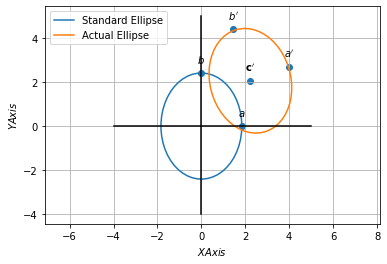
\includegraphics[width=\columnwidth]{solutions/41/20/assignment6_fig.png}
    \caption{Graphical representation of the actual curve  $40{x^2}+36{xy}+25{y^2}-196{x}-122{y}+205=0$, which represent an ellipse.}
\label{eq:solutions/41/20/myfig:1}
    \end{center}
\end{figure}

\item Trace the curve
\begin{align}
35x^2+30y^2+32x-108y-12xy+59=0 \label{eq:solutions/41/ex/given_curve_eq}
\end{align}
%
\solution
The general equation of second degree is given by
\begin{align}
ax^2+2bxy+cy^2+2dx+2ey+f=0 \label{eq:solutions/41/ex/gen_quad_eqn}
\end{align}
and can be expressed as
\begin{align}
\vec{x}^T\vec{V}\vec{x}+2\vec{u}^T\vec{x}+f=0 \label{eq:solutions/41/ex/conic_quad_eqn}
\end{align}
where
\begin{align}
\vec{V} &= \vec{V}^T = \myvec{a & b \\ b & c}
\\
\vec{u}^T &= \myvec{d & e}
\end{align}

Comparing \eqref{eq:solutions/41/ex/given_curve_eq} with \eqref{eq:solutions/41/ex/gen_quad_eqn}, we get
\begin{align}
\vec{V} &= \myvec{35  & -6 \\ -6 & 30}
\\
\vec{u}^T &= \myvec{16 & -54}
\end{align}
If $\abs{\vec{V}} > 0$, then \eqref{eq:solutions/41/ex/conic_quad_eqn} is an ellipse. 
\begin{align}
\abs{V} = 
\mydet{
35  & -6 \\ -6 & 30
}
= 1014 > 0
\end{align}
%
\eqref{eq:solutions/41/ex/conic_quad_eqn} can be expressed as
\begin{align}
\label{eq:solutions/41/ex/conic_simp_temp_nonparab_eq}
\vec{y}^T\vec{D}\vec{y} &=  \vec{u}^T\vec{V}^{-1}\vec{u} -f  &  \abs{V} &\ne 0
\\
\vec{y}^T\vec{D}\vec{y} &=  -\eta\myvec{1 & 0}\vec{y}   & \abs{V} &= 0
\label{eq:solutions/41/ex/conic_simp_temp_parab_eq}
\end{align}
with center as 
\begin{align}
    \vec{c} &= - \vec{V}^{-1}\vec{u} & \abs{V} &\ne 0
\end{align}
Calculating the center for given curve we get,
\begin{align}
    \vec{c} &= - \frac{1}{\abs{35*30 - 6*6}}\myvec{30  & 6 \\ 6 & 35}\myvec{16 \\ -54} \\
    &= \frac{1}{1014}\myvec{156 \\ -1794} \\
    &= \myvec{\frac{2}{13}  \\\frac{-23}{13}}
\end{align}

For 
\begin{align} 
\abs{\vec{V}} > 0, \quad \text{or, } \lambda_1 > 0, \lambda_2 > 0 
\end{align} 
\eqref{eq:solutions/41/ex/conic_simp_temp_nonparab_eq} becomes 
\begin{align} \lambda_1y_1^2 +\lambda_2y_1^2 = 
\vec{u}^T\vec{V}^{-1}\vec{u} -f 
\end{align} 
which is the equation of an ellipse with major and minor axes 
parameters
\begin{align} 
\sqrt{\frac{\lambda_1}{\vec{u}^T\vec{V}^{-1}\vec{u} -f}}, 
\sqrt{\frac{\lambda_2}{\vec{u}^T\vec{V}^{-1}\vec{u} -f}} \label{eq:solutions/41/ex/axes_eq}
\end{align}
The characteristic equation of $\vec{V}$ is obtained by evaluating the determinant
\begin{align}
\mydet{\lambda \vec{I}-\vec{V}} = \mydet{\lambda -35 & 6 \\ 6 & \lambda -30} &= 0
\\
\implies \lambda^2 - 65\lambda + 1014 &= 0
\label{eq:solutions/41/ex/ellipse_char_eq}
\end{align}
The eigenvalues are the roots of \eqref{eq:solutions/41/ex/ellipse_char_eq} given by
\begin{align}
\lambda_1 = 39, \lambda_2 = 26
\end{align}


Calculating the major and minor axes lengths using \eqref{eq:solutions/41/ex/axes_eq}, we get
\begin{align}
\vec{u}^T\vec{V}^{-1}\vec{u} &= \nonumber \\
&= \myvec{16 -54}\frac{1}{1014}\myvec{30 & 6 \\ 6 & 35 }\myvec{16 \\ -54} \nonumber \\
&= \frac{1}{1014}\myvec{16 & -54}\myvec{156 \\ -1794} \nonumber \\
&= 98 \nonumber \\
\vec{u}^T\vec{V}^{-1}\vec{u} -f &= 98 - 59 = 39 \\
\sqrt{\frac{\vec{u}^T\vec{V}^{-1}\vec{u} -f}{\lambda_1}} &= \sqrt{\frac{39}{39}} = 1 \\
\sqrt{\frac{\vec{u}^T\vec{V}^{-1}\vec{u} -f}{\lambda_2}} &= \sqrt{\frac{39}{26}} = \frac{\sqrt{6}}{2}
\end{align}


\begin{figure}[!ht]
\centering
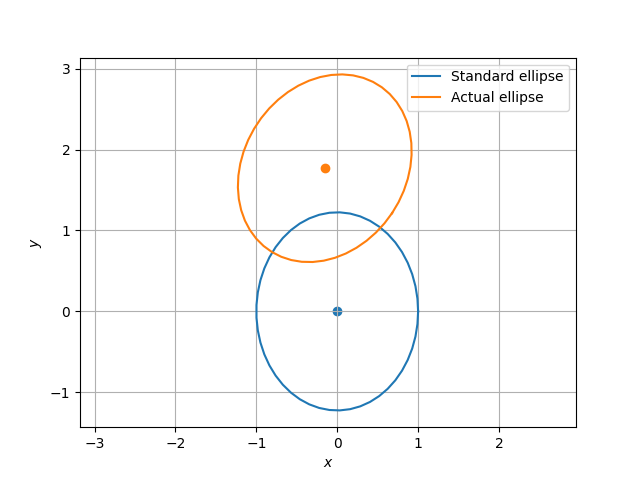
\includegraphics[width=\columnwidth]{./solutions/41/ex/Assignment7.png}

\caption{Ellipse with center \myvec{\frac{2}{13} & \frac{-23}{13}} and having the axes lengths as 1 and $\frac{\sqrt{6}}{2}$}
\label{eq:solutions/41/ex/Fig:Circle}
\end{figure}


\item Trace the curve
\begin{align}
14x^2 - 4xy + 11y^2 - 44x - 58y + 71 =0  \label{eq:solutions/41/ex1/given_curve_eq}
\end{align}

\solution
The general equation of second degree is given by
\begin{align}
ax^2+2bxy+cy^2+2dx+2ey+f=0 \label{eq:solutions/41/ex1/gen_quad_eqn}
\end{align}
and can be expressed as
\begin{align}
\vec{x}^T\vec{V}\vec{x}+2\vec{u}^T\vec{x}+f=0 \label{eq:solutions/41/ex1/conic_quad_eqn}
\end{align}
where
\begin{align}
\vec{V} &= \vec{V}^T = \myvec{a & b \\ b & c}
\\
\vec{u}^T &= \myvec{d & e}
\end{align}

Comparing \eqref{eq:solutions/41/ex1/given_curve_eq} with \eqref{eq:solutions/41/ex1/gen_quad_eqn}, we get
\begin{align}
\vec{V} &= \myvec{14  & -2 \\ -2 & 11}
\\
\vec{u}^T &= \myvec{-22 & -29}
\end{align}
If $\abs{\vec{V}} > 0$, then \eqref{eq:solutions/41/ex1/conic_quad_eqn} is an ellipse. 
\begin{align}
\abs{V} = \mydet{14 & -2 \\ -2 & 11} = 150 > 0 \label{eq:solutions/41/ex1/ellipse_proved_eq}
\end{align}
\eqref{eq:solutions/41/ex1/conic_quad_eqn} can be expressed as
\begin{align}
\label{eq:solutions/41/ex1/conic_simp_temp_nonparab_eq}
\vec{y}^T\vec{D}\vec{y} &=  \vec{u}^T\vec{V}^{-1}\vec{u} -f  &  \abs{V} &\ne 0
\\
\vec{y}^T\vec{D}\vec{y} &=  -\eta\myvec{1 & 0}\vec{y}   & \abs{V} &= 0
\label{eq:solutions/41/ex1/conic_simp_temp_parab_eq}
\end{align}
with center as 
\begin{align}
    \vec{c} &= - \vec{V}^{-1}\vec{u} & \abs{V} &\ne 0
\end{align}
Calculating the center for given curve we get,
\begin{align}
    \vec{c} &= - \frac{1}{\abs{14\times11 - \brak{-2\times-2}}}\myvec{11  & 2 \\ 2 & 14}\myvec{-22 \\ -29} \\
    &= \frac{1}{150}\myvec{300 \\ 450} \\
    &= \myvec{2 \\ 3}
\end{align}
For 
\begin{align} 
\abs{\vec{V}} > 0, \quad \text{or, } \lambda_1 > 0, \lambda_2 > 0 
\end{align} 
\eqref{eq:solutions/41/ex1/conic_simp_temp_nonparab_eq} becomes 
\begin{align} \lambda_1y_1^2 +\lambda_2y_1^2 = 
\vec{u}^T\vec{V}^{-1}\vec{u} -f 
\end{align} 
which is the equation of an ellipse with major and minor axes 
parameters
\begin{align} 
\sqrt{\frac{\lambda_1}{\vec{u}^T\vec{V}^{-1}\vec{u} -f}}, 
\sqrt{\frac{\lambda_2}{\vec{u}^T\vec{V}^{-1}\vec{u} -f}} \label{eq:solutions/41/ex1/axes_eq}
\end{align}
The characteristic equation of $\vec{V}$ is obtained by evaluating the determinant
\begin{align}
\mydet{\lambda \vec{I}-\vec{V}} = \mydet{\lambda -14 & 2 \\ 2 & \lambda -11} &= 0
\\
\implies \lambda^2 - 25\lambda + 150 &= 0
\label{eq:solutions/41/ex1/ellipse_char_eq}
\end{align}
The eigenvalues are the roots of \eqref{eq:solutions/41/ex1/ellipse_char_eq} given by
\begin{align}
\lambda_1 = 15, \lambda_2 = 10
\label{eq:solutions/41/ex1/ellipse_eval_eq}
\end{align}
The eigenvector $\vec{p}$ is defined as
\begin{align}
\vec{V} \vec{p}&= \lambda \vec{p}
\\
\implies \brak{\lambda\vec{I}-\vec{V}}\vec{p} &=0
\end{align}
where $\lambda$ is the eigenvalue.  For $\lambda_1 = 15$,
\begin{align}
\brak{\lambda_1\vec{I}-\vec{V}}
= \myvec{1 & 2 \\ 2 & 4} 
\xleftrightarrow{R_2\leftarrow R_2-2R_1}\myvec{1 & 2 \\0 & 0 }  
\\
\implies \vec{p}_1 = \frac{1}{\sqrt{5}}\myvec{2 \\ -1}
\end{align}
such that $\norm{\vec{p}_1} = 1$.  Similarly, the eigenvector corresponding to $\lambda_2$ can be obtained as
\begin{align}
 \vec{p}_2 = \frac{1}{\sqrt{5}}\myvec{1 \\ 2}
\end{align}
It is easy to verify that 
\begin{align}
\vec{V} &= \vec{P}\vec{D}\vec{P}^{-1}=\vec{P}\vec{D}\vec{P}^T \quad \because \vec{P}^{-1} = \vec{P}^{T} \label{eq:solutions/41/ex1/ellipse_spectrum_eq}
\\
\text{or, } \vec{D} &= \vec{P}^T\vec{V}\vec{P}
\end{align}
where 
\begin{align}
\vec{P} & =\myvec{\vec{p}_1 & \vec{p}_2} = \frac{1}{\sqrt{5}}\myvec{2 & 1\\ -1 & 2} \label{eq:solutions/41/ex1/ellipse_spectrum_P_eq}
\\
 \vec{D} &= \myvec{\lambda_1 & 0 \\ 0 & \lambda_2} =\myvec{15 & 0\\ 0 & 10}
\label{eq:solutions/41/ex1/eq:ellipse_spectrum_D}
\end{align}
Calculating the ellipse parameters using \eqref{eq:solutions/41/ex1/axes_eq}, we get
\begin{align}
\vec{u}^T\vec{V}^{-1}\vec{u} &= \nonumber \\
&= \myvec{-22 -29}\frac{1}{150}\myvec{11 & 2 \\ 2 &1 4 }\myvec{-22 \\ -29} \nonumber \\
&= \frac{1}{150}\myvec{300 & 450}\myvec{22 \\ 29} \nonumber \\
&= 131 \nonumber \\
\vec{u}^T\vec{V}^{-1}\vec{u} -f &= 131 - 71 = 60 \\
\sqrt{\frac{\vec{u}^T\vec{V}^{-1}\vec{u} -f}{\lambda_1}} &= \sqrt{\frac{60}{15}} = 2 \\
\sqrt{\frac{\vec{u}^T\vec{V}^{-1}\vec{u} -f}{\lambda_2}} &= \sqrt{\frac{60}{10}} = \sqrt{6}
\end{align}

Thus, the given curve is found to be an ellipse from \eqref{eq:solutions/41/ex1/ellipse_proved_eq} with center at $\myvec{2 & 3}$ and the major and minor axes lengths are calculated as $\sqrt{6}$, $2$. An ellipse with these parameters along with one having center as origin are plotted as shown.

\begin{figure}[!ht]
\centering
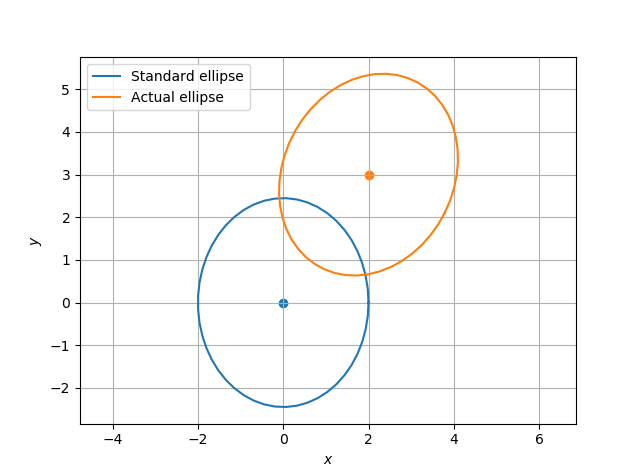
\includegraphics[width=\columnwidth]{./solutions/41/ex1/assignment_6_figure.png}
\caption{Ellipse with center (2 3) and having the axes lengths as $\sqrt{6}$ and 2 along with an ellipse with center as origin}
\label{eq:solutions/41/ex1/Fig:Ellipse}
\end{figure}

\item Trace the following 
\begin{align}
    x^2-3xy+y^2+10x-10y+21=0 \label{eq:solutions/41/ex2/eq 1}
\end{align}
%
\solution
The given quadratic equation can be written in the matrix form as
\begin{align}
    \vec{x}^T\myvec{1&-\frac{3}{2}\\-\frac{3}{2}&1}\vec{x}+2\myvec{5&-5}\vec{x}+21=0\label{eq:solutions/41/ex2/eq:1}
\end{align}
Calculating the parameters,we get
\begin{align}
    \mydet{\vec{V}}=\mydet{1&-\frac{3}{2}\\-\frac{3}{2}&1}=-\frac{5}{4}
\end{align}
Since, $\mydet{\vec{V}} < 0$, therefore the given  equation represents a hyperbola.\par
The characteristic equation of $\vec{V}$ will be
\begin{align}
    \mydet{\vec{V}-\lambda\vec{I}}&=\mydet{1-\lambda&-\frac{3}{2}\\-\frac{3}{2}&1-\lambda}=0\\
    &\implies 4\lambda^2-8\lambda-5 =0 \\
   &\implies\lambda_1=\frac{5}{2},\lambda_2=-\frac{1}{2}\label{eq:solutions/41/ex2/eq 2}
\end{align}
The eigen vector $\vec{p}$ is given by
\begin{align}
 \vec{V}\vec{p}=\lambda\vec{p}
\end{align}
\begin{align}
  \implies{\vec{V}-\lambda\vec{I}} \vec{p}=0 \label{eq:solutions/41/ex2/eq 3} 
\end{align}
For $\lambda_1 = \frac{5}{2} $
\begin{align}
\vec{V}-\lambda\vec{I}= \myvec{1-\frac{5}{2}&-\frac{3}{2}\\-\frac{3}{2}&1-\frac{5}{2}}
    \end{align}
    \begin{align}
 =\myvec{-\frac{3}{2}&-\frac{3}{2}\\-\frac{3}{2}&-\frac{3}{2}}
    \end{align}
    \begin{align}
    \myvec{-\frac{3}{2}&-\frac{3}{2}\\-\frac{3}{2}&-\frac{3}{2}}\xleftrightarrow{R_2=R_2-R_1}\myvec{-\frac{3}{2}&-\frac{3}{2}\\ 0 &0}
\end{align}
 \begin{align}
    \xleftrightarrow{R_1=R_1/-\frac{3}{2}}\myvec{1&1\\ 0 &0}\label{eq:solutions/41/ex2/eq 4}
   \end{align}
Substituting \eqref{eq:solutions/41/ex2/eq 4} in \eqref{eq:solutions/41/ex2/eq 3} we get 
\begin{align}
   \vec{p_1}=\myvec{-1\\1}
\end{align}
Therefore the normalized eigen vector will be
\begin{align}
    \vec{p_1}=\myvec{-\frac{1}{\sqrt{2}}\\\frac{1}{\sqrt{2}}}
\end{align}
For $\lambda_2 = -\frac{1}{2} $
\begin{align}
\vec{V}-\lambda\vec{I}= \myvec{1+\frac{1}{2}&-\frac{3}{2}\\-\frac{3}{2}&1+\frac{1}{2}}
    \end{align}
    \begin{align}
 =\myvec{\frac{3}{2}&-\frac{3}{2}\\-\frac{3}{2}&-\frac{3}{2}}
    \end{align}
    \begin{align}
    \myvec{-\frac{3}{2}&-\frac{3}{2}\\-\frac{3}{2}&-\frac{3}{2}}\xleftrightarrow{R_2=R_2+R_1}\myvec{-\frac{3}{2}&-\frac{3}{2}\\ 0 &0}
\end{align}
 \begin{align}
    \xleftrightarrow{R_1=R_1/\frac{3}{2}}\myvec{1&-1\\ 0 &0}\label{eq:solutions/41/ex2/eq 5}
   \end{align}
Substituting \eqref{eq:solutions/41/ex2/eq 5} in \eqref{eq:solutions/41/ex2/eq 3} we get 
\begin{align}
   \vec{p_2}=\myvec{1\\1}
\end{align}
Therefore the normalized eigen vector will be
\begin{align}
    \vec{p_2}=\myvec{\frac{1}{\sqrt{2}}\\\frac{1}{\sqrt{2}}}
\end{align}
Eigen decomposition\\ 
Since $\vec{V}=\Vec {V}^T$there exists an orthogonal matrix P such that
\begin{align}
    \vec{P}\vec{P}^T=\vec{I}
\end{align}
\begin{align}
    \vec{P}\vec{V}\vec{P}^T=\vec{D}= diag\brak{\lambda_1 \lambda_2}
\end{align}
or equivalently
\begin{align}
    \vec{V}= \vec{P} \vec{D} \vec{P}^T
\end{align}
As
\begin{align}
  \vec{P}=\myvec{p_1&p_2}= \myvec{-\frac{1}{\sqrt{2}}&\frac{1}{\sqrt{2}}\\\frac{1}{\sqrt{2}}& \frac{1}{\sqrt{2}}}\\
   \vec{D}=\myvec{\lambda_1&0\\0&\lambda_2}\\
   \implies 
   \vec{D}=\myvec{\frac{5}{2}&0\\0&-\frac{1}{2}} \label{eq:solutions/41/ex2/eq 6}\\
    \vec{C}=-\vec{V}^{-1}\vec{u}\\
    \implies\vec{C} =\myvec{-\frac{4}{5}&-\frac{6}{5}\\-\frac{6}{5}&-\frac{4}{5}} \myvec{-5\\ 5}\\
   = \myvec{-2\\2}
\end{align}
$\therefore$ Centre C is given by: 
\begin{align}
  \myvec{-2\\2}
%\label{eq:solutions/41/ex2/eq 6}
 \end{align}
 Now Equation \eqref{eq:solutions/41/ex2/eq 1} can be written as
\begin{align}
    \vec{y}^T\vec{D}\vec{y}=\vec{u}^T \vec {V}^{-1}\vec {u}-\vec {f}\\
\end{align}
where y is given by:
\begin{align}
     \vec{y}= \vec{P}^T\brak{\vec{x}-\vec{c}}
\end{align}
So 
\begin{align}
   \vec{y}^T\myvec{\frac{5}{2}&0\\0&-\frac{1}{2}}\vec{y}=-1\\
   \implies \vec{y}^T\myvec{\frac{5}{2}&0\\0&-\frac{1}{2}}\vec{y}+1=0
\end{align}
\begin{figure}[ht!]
	\centering
	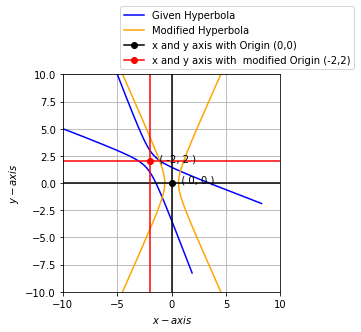
\includegraphics[width=\columnwidth]{./solutions/41/ex2/hyberbola.png}
	\caption{Hyperbola plot when origin is shifted}
	\label{eq:solutions/41/ex2/myfig}
\end{figure}


\end{enumerate}
